\subsection{分式环的整闭包}

设 A 是环，R 是 A-代数，S 是 A 的乘性子集。回忆（第 II 章，§ 2，第 8 节），\(\mathbf{S}^{-1}\mathbf{R}\) 具有典范的 \(\mathbf{S}^{-1}\mathbf{A}\) -代数结构。

命题 16. 设 A 是环，R 是 A-代数，A' 是 A 在 R 中的整闭包，S 是 A 的乘性子集。则 \(\mathbf{S}^{-1}\mathbf{A}\) 在 \(\mathbf{S}^{-1}\mathbf{R}\) 中的整闭包是 \(\mathbf{S}^{-1}\mathbf{A}'\) 。

设 \(b / s\) 是 \(S^{-1}A'\) 的元素（ \(s \in S, b \in A'\) ）。由于图

\pandocbounded{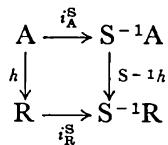
\includegraphics[keepaspectratio]{images/part002_55e4c379.jpg}}

是交换的，\(b / 1\) 在 \(S^{-1}A\) 上是整的（第 1 节，命题 2）。由于 \(1 / s \in S^{-1}A\) ，故 \(b / s = (b / 1)(1 / s)\) 在 \(S^{-1}A\) 上是整的。

反之，设 \(r / t\)（ \(r \in \mathbb{R}\) ，\(t \in \mathbb{S}\) ）是 \(\mathbf{S}^{-1}\mathbf{R}\) 中在 \(\mathbf{S}^{-1}\mathbf{A}\) 上整的元素；则 \(r / 1 = (t / 1)(r / t)\) 在 \(\mathbf{S}^{-1}\mathbf{A}\) 上是整的。于是存在形如

\[
(r / 1) ^ {n} + (a _ {1} / s) (r / 1) ^ {n - 1} + \dots + (a _ {n} / s) = 0,
\]

的关系式，其中 \(a_{i} \in \mathbf{A}\)（ \(1 \leqslant i \leqslant n\) ），\(s \in \mathbf{S}\) 。这个关系式也可以写成

\[
(s r ^ {n} + a _ {1} r ^ {n - 1} + \dots + a _ {n}) / s = 0
\]

从而存在 \(s' \in S\) 使得 \(s'^{n}(sr^{n} + a_{1}r^{n-1} + \cdots + a_{n}) = 0\) ；由此推出 \((s'sr)^{n} + s'a_{1}(s'sr)^{n-1} + \cdots + s'^{n}s^{n-1}a_{n} = 0\) 。因此按定义有 \(s'sr \in A'\) ，从而 \(r/1 \in S^{-1}A'\) ，且 \(r/t \in S^{-1}A'\) 。

推论 1. 设 A 是整环，A' 是它的整闭包，S 是 A 的乘性子集且 \(0 \notin S\) 。则 \(S^{-1}A\) 的整闭包是 \(S^{-1}A'\) 。

A 的分式域 R 也是 \(S^{-1}A\) 的分式域，因为 \(0 \notin S\) （第 II 章，§ 1，第 1 节，注 7）；对 R 应用命题 16 即得。

推论 2. 设 A 是整环，K 是它的分式域，R 是 K 上的代数，B 是 A 在 R 中的整闭包。R 中在 K 上代数的元素（第 1 节，例 1）恰是形如 \(a^{-1}b\) 的元素，其中 \(b \in \mathbf{B}\)，\(a \in \mathbf{A}\)，\(a \neq 0\) ；若 L 是 K 在 R 中的代数闭包，则存在包含在 B 中的 L 在 K 上的基。

第一个断言由命题 16 应用于 \(\mathbf{S} = \mathbf{A} - \{0\}\) 的情形而得。若 \((x_{i})_{i\in I}\) 是 \(\mathbf{L}\) 在 \(\mathbf{K}\) 上的一组基，则对每个 \(i\in I\) 存在元素 \(a_{i}\neq 0\) 属于 \(\mathbf{A}\) ，使得 \(a_{i}x_{i}\in \mathbf{B}\) ；于是 \((a_{i}x_{i})_{i\in I}\) 也是 \(\mathbf{L}\) 在 \(\mathbf{K}\) 上的基。

推论 3. 设 A 是整环，\(\Omega\) 是 A 的极大理想组成的集。为使 A 是整闭的，必须而且只需对所有 \(\mathfrak{m} \in \Omega\) ，\(\mathbf{A}_{\mathfrak{m}}\) 都是整闭的。

由推论 1 可知该条件是必要的。该条件也是充分的，因为 \(\mathbf{A} = \bigcap_{m \in \Omega} \mathbf{A}_m\)（第 II 章，§3，第 3 节，公式 (2)），故只需应用第 2 节命题 8 的推论即可。

推论 4. 设 A 是整环，K 是它的分式域，S 是 A 的乘性子集且 \(0 \notin S\) 。

\begin{enumerate}
\def\labelenumi{(\roman{enumi})}
\item
  设 B 是 K 的子环且在 A 上是整的，f 是 A-模 B/A 的零化子。则 \(S^{-1}f\) 包含在 \((S^{-1}A)\) -模 \(S^{-1}B/S^{-1}A\) 的零化子之中，且当 B 是有限生成 A-模时等于这个零化子。
\item
  设 A' 是 A 的整闭包。为使 \(S^{-1}A\) 整闭，只需 A-模 A'/A 的零化子 f 与 S 相交。若 A' 是有限生成 A-模，这个条件也是必要的。
\setcounter{enumi}{0}
\item
  由于 \(\mathfrak{f}\mathbf{B} \subset \mathbf{A}\) ，有 \((\mathrm{S}^{-1}\mathfrak{f})(\mathrm{S}^{-1}\mathbf{B}) \subset \mathrm{S}^{-1}\mathbf{A}\) ，因而 \(\mathrm{S}^{-1}\mathfrak{f}\) 包含在 Ann \((\mathrm{S}^{-1}\mathrm{B} / \mathrm{S}^{-1}\mathrm{A})\) 之中。若 \(\mathbf{B}\) 是有限生成 A-模，则等式 \(\mathrm{S}^{-1}\mathfrak{f} = \operatorname{Ann}(\mathrm{S}^{-1}\mathrm{B} / \mathrm{S}^{-1}\mathrm{A})\) 是第 II 章 § 2 第 4 节公式 (9) 的特殊情形，这里 \(\mathrm{S}^{-1}\mathrm{B} / \mathrm{S}^{-1}\mathrm{A}\) 典范地等同于 \(\mathrm{S}^{-1}(\mathrm{B} / \mathrm{A})\) 。
\item
  由推论 1，\(\mathbf{S}^{-1}\mathbf{A}'\) 是 \(\mathbf{S}^{-1}\mathbf{A}\) 的整闭包。由于关系 \(\mathfrak{f} \cap \mathbf{S} \neq \varnothing\) 与 \(\mathbf{S}^{-1}\mathfrak{f} = \mathbf{S}^{-1}\mathbf{A}\) 等价（第 II 章，§ 2，第 5 节，注），(ii) 是 (i) 的直接推论。
\end{enumerate}

若 B 是 K 的子环且在 A 上是整的，则 B/A 的零化子 f（按定义等于传递子 A: B（第 I 章，§ 2，第 10 节））有时称为 B 在 A 中的导子。

推论 5. 设 A 是整环，A' 是它的整闭包，f 是 A-模 A'/A 的零化子。假设 A' 是有限生成 A-模。则使 A \(_{p}\) 不是整闭的 A 的素理想 p 恰是包含 f 的那些素理想。

这由推论 4 (ii) 应用于 S = A - p 立即得出。

注意，在推论 5 的假设之下 f ≠ 0，因为 A' 是有限生成 A-模，且 K/A（K 是 A 的分式域）的每个元素的零化子都 ≠ 0。

* 在代数几何中，推论 5 与上面的注表明：仿射簇 V 的非正规点组成一个异于 V 的闭集。*

\subsection{整元的范数与迹}

命题 17. 设 A 是环，B 是（交换）A-代数，X 是 B 上的 n 阶方阵；则下列性质等价：

\begin{enumerate}
\def\labelenumi{(\alph{enumi})}
\item
  \(X\) 在 A 上是整的。
\item
  存在 \(\mathbf{M}\) （\(\mathbf{B}^n\) 的一个有限生成子 A-模），使得 \(X.x\in \mathbf{M}\) 对所有 \(x\in \mathbf{M}\) 成立，且 \(\mathbf{M}\) 是 B-模 \(\mathbf{B}^n\) 的一个生成系。
\item
  \(X\) 的特征多项式的系数在 \(\mathbf{A}\) 上是整的。
\end{enumerate}

  若 \(\chi(T) = \det(T.1 - X)\) 是 \(X\) 的特征多项式，则 Cayley-Hamilton 定理表明 \(\chi(X) = 0\)（《代数》第 VII 章，§ 5，第 4 节，注 1），且由于 \(\chi\) 是首一多项式，由第 1 节命题 6 知 (c) 蕴含 (a)。

  其次假设 (a) 成立。若 \((e_i)_{1 \leqslant i \leqslant n}\) 是 \(B^n\) 的典范基，则由诸 \(X^k \cdot e_i\)（ \(1 \leqslant i \leqslant n, k \geqslant 0\) ）生成的 B 的子 A-模 M 是有限生成 A-模，因为 A-代数 A[X] 是有限生成 A-模（第 1 节，定理 1）；由于 M 包含诸 \(e_i\) ，可见 (a) 蕴含 (b)；其逆是第 1 节定理 1 条件 \((E_{\mathrm{III}})\) 的推论。

  最后证明 (a) 蕴含 (c)；由于 X 在 A 上整，从而更加在多项式环 A[T] 上整，故 T.1 - X 也在 A[T] 上整，且由第 3 节命题 12 可见，问题可化归（把 X 换成 T.1 - X，把 A 换成 A[T]）为证明：若 X 在 A 上整，则 \(d = \det(X)\) 是 B 中在 A 上整的元素。而上面已经看到，由 X 定义的 \(B^{n}\) 的自同态 u 使一个包含诸 \(e_{i}\) 的有限生成子 A-模 M 保持稳定；于是 n-向量 \(x_{1} \wedge x_{2} \wedge \cdots \wedge x_{n}\) ，其中 \(x_{i} \in M\)

（ \(1 \leqslant i \leqslant n\) ）的这些向量于是在 \(\bigwedge (\mathbf{B}^n)\) 中生成一个包含 \(e_1 \wedge e_2 \wedge \cdots \wedge e_n\) 的有限生成子 A-模，它在 \(\bigwedge^n u\) 之下稳定，换言之在比率为 \(d\) 的位似之下稳定；由于

\[
e _ {1} \wedge e _ {2} \wedge \dots \wedge e _ {n}
\]

在 B 中的零化子仅为 0，故第 1 节定理 1 的条件 \((\mathbf{E}_{\mathrm{III}})\) 证明 \(d\) 在 A 上是整的。

推论 1. 设 A 是整环，K 是它的分式域，K' 是有限维 K-代数（不一定交换）。若 \(x \in \mathbf{K}'\) 在 A 上是整的，则特征多项式 \(\mathrm{Pc}_{\mathbf{K}' / \mathbf{K}}(x; \mathbf{X})\)（《代数》第 VIII 章，§ 12，第 2 节）的系数在 A 上是整的。

若 \(z \mapsto M(z)\) 是代数 \(\mathbf{K}'\) 的正则表示（看作矩阵表示；参见《代数》第 VIII 章，§ 13），则 \(\mathrm{Pc}_{\mathbf{K}' / \mathbf{K}}(x; \mathbf{X})\) 按定义就是矩阵 \(M(x)\) 的特征多项式；若 \(x\) 在 \(\mathbf{A}\) 上是整的，则矩阵 \(M(x)\) 在 \(\mathbf{A}\) 上是整的（第 1 节，命题 2），故只需应用命题 17。

推论 2. 在与推论 1 相同的假设与记号下，\(\mathrm{Tr}_{\mathbf{K}^{\prime}/\mathbf{K}}(x)\) 与 \(\mathbf{N}_{\mathbf{K}^{\prime}/\mathbf{K}}(x)\) 都在 A 上是整的。

\(\mathrm{Tr}_{\mathbf{K}^{\prime}/\mathbf{K}}(x)\) 与 \(\mathrm{N}_{\mathbf{K}^{\prime}/\mathbf{K}}(x)\) 是 \(\mathrm{Pc}_{\mathbf{K}^{\prime}/\mathbf{K}}(x;\mathbf{X})\) 的系数（《代数》第 VIII 章，§ 12，第 1 节，公式 (4)），至多相差一个符号，从而是整的。

注 (1) 若 \(\mathbf{K}'\) 是 \(\mathbf{K}\) 上的中心单代数，且 \(x \in \mathbf{K}'\) 在 \(\mathbf{A}\) 上是整的，则 \(x\) 的约化特征多项式（《代数》第 VIII 章，§ 12，第 3 节）的系数在 \(\mathbf{A}\) 上是整的。因为这个多项式有一个方幂等于 \(\mathrm{Pc}_{\mathbf{K}' / \mathbf{K}}(x; \mathbf{X})\)（同前，命题 8），故只需应用命题 17 及第 3 节命题 11。

命题 18. 设 A 是整闭整环，K 是它的分式域，K' 是有限维可分 K-代数（《代数》第 VIII 章，§7，第 5 节），A' 是 A 在 K' 中的整闭包。则 A' 包含在一个有限生成 A-模之中。

该命题可由下面更精确的引理得出：

引理 3. 在命题 18 的假设下，设 \((w_{1},\ldots ,w_{n})\) 是 \(\mathbf{K}'\) 在 \(\mathbf{K}\) 上的包含在 \(\mathbf{A}'\) 中的一组基（第 5 节，命题 16 的推论 2）；则存在唯一的一组基 \((w_{1}^{*},\dots ,w_{n}^{*})\) （\(\mathbf{K}'\) 在 \(\mathbf{K}\) 上的基），使得 \(\mathrm{Tr}_{\mathbf{K}' / \mathbf{K}}(w_i w_j^*) = \delta_{ij}\) （Kronecker 指标）；若 \(d = \mathrm{D}_{\mathbf{K}' / \mathbf{K}}(w_1,\dots ,w_n)\) 是基 \((w_{1},\dots ,w_{n})\) 的判别式（《代数》第 IX 章，§ 2），则 \(d\neq 0\) ，且

\[
\sum_ {i = 1} ^ {n} \mathrm{A} w _ {i} \subset \mathrm{A} ^ {\prime} \subset \sum_ {i = 1} ^ {n} \mathrm{A} w _ {i} ^ {*} \subset d ^ {- 1} \left(\sum_ {i = 1} ^ {n} \mathrm{A} w _ {i}\right).\tag{2}
\]

特别地，若 \(d\) 是 \(\mathbf{A}\) 的可逆元，则 \(\mathbf{A}'\) 是自由 \(\mathbf{A}\) -模，以 \((w_1, \ldots, w_n)\) 为基。

由于 \(\mathbf{K}'\) 是可分 K-代数，故 \(d \neq 0\)（《代数》第 IX 章，§2，命题 5），且 K-双线性形式

\[
(x, y) \mapsto \operatorname{Tr} _ {\mathbf {K} ^ {\prime} / \mathbf {K}} (x y)
\]

在 \(\mathbf{K}'\) 上是非退化的（同前，命题 4）；这就表明了基 \((w_{i}^{*})_{1\leqslant i\leqslant n}\) 的存在性与唯一性（《代数》第 IX 章，§1，第 6 节，命题 6 的推论）。在这样的约定下，(2) 的第一个包含关系是

显然的。设 \(x\) 是 \(\mathbf{A}'\) 的元素；记 \(x = \sum_{i=1} \xi_i w_i^*\) ，其中 \(\xi_i \in \mathbf{K}\) ；对每个 \(i\) ，\(\xi_i = \mathrm{Tr}_{\mathbf{K}' / \mathbf{K}}(xw_i)\) ，故 \(\xi_i\) 在 \(\mathbf{A}\) 上是整的（命题 17 的推论 2），且由于 \(\mathbf{A}\) 是整闭的，有 \(\xi_i \in \mathbf{A}\) （\(1 \leqslant i \leqslant n\)） ；这就证明了第二个

包含关系 (2)。最后，记 \(w_{j}^{*} = \sum_{l=1}^{n} \alpha_{jl} w_{l}\) ，其中 \(\alpha_{jl} \in \mathbf{K}\) ；则 \(\sum_{i=1}^{n} \alpha_{ji} \mathrm{Tr}_{\mathbf{K}'/\mathbf{K}}(w_i w_k) = \delta_{jk}\) 对所有 \(j\) 与 \(k\) 成立；Cramer 公式表明诸 \(\alpha_{ji}\) 属于 \(d^{-1}\mathbf{A}\) ，由此得第三个包含关系 (2)。最后的断言由 (2) 立即得出，因为在此情形 (2) 给出 \(\mathbf{A}' = \sum_{i=1}^{n} \mathbf{A}w_i\) 。

在下面两个推论中，假设与记号均取命题 18 者。

推论 1. 若 A 是 Noether 环，则 A-模 A' 是有限生成的，特别地，环 A' 是 Noether 环。

A' 是一个有限生成 A-模的子模。

推论 2. 若 A 是主理想整环，则 A' 是秩为 n 的自由 A-模。此时自由 A-模的每个子模都是自由的（《代数》第 VII 章，§ 3，定理 1）。

推论 3. 设 E 是有理数域 Q 的 n 次扩张。有理整数环 Z 在 E 中的整闭包的加法群是秩为 n 的自由交换群。

Z 是整闭的（第 3 节，命题 10），且由于 Q 的特征为 0，E 是可分的。因此推论 2 可以应用于 A = Z，K = Q，K' = E 的情形。

注 (2). 若不假设 \(\mathbf{K}'\) 在 \(\mathbf{K}\) 上可分，则推论 1 的结论不一定成立，即使 \(\mathbf{K}'\) 是 \(\mathbf{K}\) 的扩域（习题 20）也是如此。另一方面，若 \(\mathbf{A}\) 是有限生成的整 \(\mathbf{K}_0\) -代数，其中 \(\mathbf{K}_0\) 是域，则正如我们将在 §3 第 2 节定理 2 中看到的，\(\mathbf{A}\) 在其分式域的任意有限次扩张中的整闭包是有限生成 \(\mathbf{A}\) -模，并且是 Noether 环。

\pandocbounded{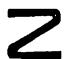
\includegraphics[keepaspectratio]{images/part002_ebb97593.jpg}}

\subsection{整闭代数中的纯量扩张}

命题 19. 设 \(k\) 是域，\(L\) 是 \(k\) 的可分扩张，\(R\) 是整闭的 \(k\) -代数。若环 \(L \otimes_k R\) 是整环，则它是整闭的。

设 K 是 R 的分式域；由于 k 是域，\(L \otimes_{k} R\) 典范地等同于 \(L \otimes_{k} K\) 的子 k-代数，而 L 与 R 典范地等同于 \(L \otimes_{k} R\) 的子 k-代数。此外，由于 R 的元素 \(s \neq 0\) 不是 R 中的零因子，且 L 在 k 上平坦（第 I 章，§2，第 3 节），故 \(1 \otimes s\) 不是 \(L \otimes_{k} R\) 中的零因子；把 s 与 \(1 \otimes s\) 等同，于是可以看出，若 S = R - \{0\}，则 \(L \otimes_{k} K\) 等同于 \(S^{-1}(L \otimes_{k} K)\) ；由于假设 \(L \otimes_{k} R\) 是整环，\(L \otimes_{k} K\) 便等同于 \(\Omega\) ——\(L \otimes_{k} R\) 的分式域——的子环。

\begin{enumerate}
\def\labelenumi{(\arabic{enumi})}
\tightlist
\item
  假设 \(\mathbf{L}\) 是 \(k\) 的有限扩张；则 \(\mathbf{L} \otimes_k \mathbf{K}\) 是 \(\mathbf{K}\) 上的有限秩代数，且由假设没有零因子；因此它是域（《代数》第 V 章，§2，第 1 节，命题 1），从而在此情形它就是 \(\Omega\) ，即 \(\mathbf{L} \otimes_k \mathbf{R}\) 的分式域。设 \((w_1, \ldots, w_n)\) 是 \(\mathbf{L}\) 在 \(k\) 上的基，它因而也是 \(\mathbf{L} \otimes_k \mathbf{K}\) 在 \(\mathbf{K}\) 上的基。存在一组基 \((w_1^*, \ldots, w_n^*)\) （\(\mathbf{L}\) 的基），使得 \(\mathrm{Tr}_{\mathrm{L/k}}(w_i w_j^*) = \delta_{ij}\) （第 6 节，引理 3）；每个 \(z \in \mathbf{L} \otimes_k \mathbf{K}\) 都可唯一地写成 \(z = \sum_{i=1}^{n} a_i w_i\) ，其中 \(a_i \in \mathbf{K}\) ；于是
\end{enumerate}

\[
\operatorname{Tr} _ {(\mathrm{L} \otimes \mathrm{K}) / \mathrm{K}} (z w _ {j} ^ {*}) = \sum_ {i = 1} ^ {n} a _ {i} \operatorname{Tr} _ {(\mathrm{L} \otimes \mathrm{K}) / \mathrm{K}} (w _ {i} w _ {j} ^ {*})
\]

又由于在 L 中迹 \(\mathrm{Tr}_{(L\otimes K)/K}\) 与 \(\mathrm{Tr}_{L/K}\) 一致（《代数》第 VIII 章，§ 12，第 2 节，公式 (13)），最终得 \(\mathrm{Tr}_{(L\otimes K)/K}(zw_j^*) = a_j\) ，\(1 \leqslant j \leqslant n\) 。另一方面注意 L 的元素在 \(k\) 上是整的，从而也在 R 上是整的（第 1 节，命题 2 的推论 1）；因此（第 1 节，命题 5）\(\mathbf{L} \otimes_k \mathbf{R}\) 在 R 上是整的。在这样的约定下，设 \(z \in \mathbf{L} \otimes_k \mathbf{K}\) 在 \(\mathbf{L} \otimes_k \mathbf{R}\) 上是整的；则 \(z\) 也在 R 上是整的（第 1 节，命题 6），从而 \(zw_j^*\) 亦然，于是 \(a_j = \mathrm{Tr}_{(L\otimes K)/K}(zw_j^*)\) （\(1 \leqslant j \leqslant n\)）也在 R 上是整的（第 6 节，命题 17 的推论 2）。由于 R 是整闭的，\(a_j \in \mathbf{R}\) 对所有 \(j\) 成立，从而 \(z \in \mathbf{L} \otimes_k \mathbf{R}\) ，这就证明了此情形下的命题。

\begin{enumerate}
\def\labelenumi{(\arabic{enumi})}
\setcounter{enumi}{1}
\tightlist
\item
  现在假设 \(\mathbf{L}\) 是 \(k\) 的有限生成的可分扩张；则存在 \((x_1, \ldots, x_d)\) ，它是 \(\mathbf{L}\) 在 \(k\) 上的分离超越基（《代数》第 V 章，§ 9，第 3 节，定理 2）；由于 \(\mathbf{L}\) 与 \(\mathbf{K}\) 在 \(k\) 上于域 \(\Omega\) 中代数不相交（《代数》第 V 章，§ 5，第 4 节），故诸 \(x_i\) 在 \(\mathbf{K}\) 上代数无关；从而 \(\mathrm{R}[x_1, \ldots, x_d]\) 是整闭的（第 3 节，命题 13 的推论 2）。设 \(\mathbf{T}\) 是由 \(\neq 0\) 的元素组成的集（环 \(\mathbf{A} = k[x_1, \ldots, x_d] \subset \mathbf{L}\) 的），于是域 \(k_1 = k(x_1, \ldots, x_d) \subset \mathbf{L}\) 等于 \(\mathbf{T}^{-1} k[x_1, \ldots, x_d]\) ；则
\end{enumerate}

\[
\begin{array}{r l} k _ {1} \otimes_ {k} \mathrm{R} & = (\mathrm{T} ^ {- 1} \mathrm{A}) \otimes_ {k} \mathrm{R} = \mathrm{T} ^ {- 1} \mathrm{A} \otimes_ {\mathrm{A}} (\mathrm{A} \otimes_ {k} \mathrm{R}) = \mathrm{T} ^ {- 1} (\mathrm{A} \otimes_ {k} \mathrm{R}) \\ & = \mathrm{T} ^ {- 1} \mathrm{R} [ x _ {1}, \dots , x _ {d} ] \end{array}
\]

（由张量积的结合律），因此这个整环是整闭的（第 5 节，命题 16 的推论 1）。但 \(\mathbf{L} \otimes_k \mathbf{R}\) 等同于 \(\mathbf{L} \otimes_{k_1} (k_1 \otimes_k \mathbf{R})\) ，且按定义 \(\mathbf{L}\) 是 \(k_1\) 的有限可分扩张；于是由 (1) 可得 \(\mathbf{L} \otimes_k \mathbf{R}\) 是整闭的。

\begin{enumerate}
\def\labelenumi{(\arabic{enumi})}
\setcounter{enumi}{2}
\tightlist
\item
  一般情形。若 z 是 \(\Omega\) 中在 \(L \otimes_{k} R\) 上整的元素，则它满足形如 \(z^{m} + b_{1}z^{m-1} + \cdots + b_{m} = 0\) 的关系式，其中诸 \(b_{i}\) 属于 \(L \otimes_{k} R\) ；于是存在 L 在 k 上的有限生成子扩张 \(L'\) ，使得诸 \(b_{i}\) 属于 \(L' \otimes_{k} R\) （\(1 \leqslant i \leqslant m\)），且 z 属于 \(L' \otimes_{k} K\) 。于是由 (2) 得 \(z \in L' \otimes_{k} R\) ，从而 \(L \otimes_{k} R\) 是整闭的。
\end{enumerate}

* 设 V 是不可约仿射代数簇，k 是 V 的定义域，R 是 k 上定义的 V 上的正则函数所成的环；若 R 是整闭的，则称 V 在 k 上是正规的；命题 19 表明，若 V 在 k 上正规，则它在 k 的每个可分扩张 L 上仍是正规的。*

推论. 设 \(k\) 是域，\(\mathbf{R}\) 与 \(\mathbf{S}\) 是两个整闭的 \(k\) -代数。假设环 \(\mathbf{R} \otimes_k \mathbf{S}\) 是整环，且分式域 \(\mathbf{K}\) 与 \(\mathbf{L}\) （分别为 \(\mathbf{R}\) 与 \(\mathbf{S}\) 的分式域）在 \(k\) 上可分。则环 \(\mathbf{R} \otimes_k \mathbf{S}\) 是整闭整环。

由于 R 与 S 等同于 \(R \otimes_{k} S\) 的子代数，K 与 L 等同于 \(\Omega\) ——\(R \otimes_{k} S\) 的分式域——的在 k 上线性不相交的子域（《代数》第 V 章，§2，第 3 节，命题 5）。于是由命题 19 可知 \(R \otimes_{k} L\) 与 \(K \otimes_{k} S\) 都是整闭整环；由于它们的交是 \(R \otimes_{k} S\) （第 I 章，§2，第 6 节，命题 7），故 \(R \otimes_{k} S\) 是整闭整环（第 2 节，命题 8 的推论）。

* 给定 k 上定义的两个不可约仿射簇 V，W，它们的乘积 \(V \times W\) 是仿射簇，且 \(V \times W\) 上的正则函数环等同于 V 上正则函数环与 W 上正则函数环在 k 上的张量积。命题 19 的推论表明，若 V 与 W 都在 k 上正规，则 \(V \times W\) 在 k 上正规。*

\subsection{分次环上的整元}

本节考虑的分次都是 Z 型的；若 A 是分次环且 \(i \in Z\) ，则 \(A_{i}\) 表示环 A 的次数为 i 的齐次元组成的集。

设 A 是分次环，B 是分次 A-代数。设 x 是 B 的在 A 上整的齐次元；则存在关系式

\[
x ^ {n} + a _ {1} x ^ {n - 1} + \dots + a _ {n} = 0 \quad \text { where } \quad a _ {i} \in A \quad \text { for } \quad 1 \leqslant i \leqslant n.\tag{3}
\]

设 \(m = \deg(x)\) ，并设 \(a_i'\) 是 \(mi\) 次齐次分量（\(a_i\) 的）（ \(1 \leqslant i \leqslant n\) ）；则显然

\[
x ^ {n} + a _ {1} ^ {\prime} x ^ {n - 1} + \dots + a _ {n} ^ {\prime} = 0\tag{4}
\]

换言之，x 满足一个系数为齐次元的整依赖方程。

用 \(\mathbf{A}[\mathbf{X},\mathbf{X}^{-1}]\) 表示分式环 \(\mathbf{S}^{-1}\mathbf{A}[\mathbf{X}]\) ，即单未定元多项式环 \(\mathbf{A}[\mathbf{X}]\) 的分式环，其中 \(\mathbf{S}\) 是 \(\mathbf{A}[\mathbf{X}]\) 中由方幂 \(\mathbf{X}^n\) （\(\mathbf{X}\) 的方幂， \(n\geqslant 0\) ）组成的乘性子集；由于 \(\mathbf{X}\) 不是 \(\mathbf{A}[\mathbf{X}]\) 中的零因子，立即可见诸 \(\mathbf{X}^i\)（ \(i\in \mathbf{Z}\) ）构成 \(\mathbf{A}\) 上 A-模 \(\mathbf{A}[\mathbf{X},\mathbf{X}^{-1}]\) 的一组基。对每个元素 \(a\in \mathbf{A}\) ，其齐次分量为 \(a_{i}\)（ \(i\in \mathbf{Z}\) ），我们记

\iffalse
\begin{description}
\tightlist
\item[\$\$]
j \_ \{\mathbf {A}\} (a) = \sum\_ \{i \in \mathbf {Z}\} a \_ \{i\} \mathbf {X} \^{} \{i\} \in \mathrm{A} {[} \mathbf {X}, \mathbf {X} \^{} \{- 1\} {]}\tag{5} \$\$
\end{description}
\fi

\[
:j_{A}(a) = \sum_{i \in \mathbf{Z}} a_{i} \mathbf{X}^{i} \in \mathbf{A}[\mathbf{X},\mathbf{X}^{-1}]\tag{5}
\]

立即可见 \(j_{A}: A \to A[X, X^{-1}]\) 是单的环同态。

命题 20. 设 \(\mathbf{A} = \bigoplus_{i\in \mathbf{Z}}\mathbf{A}_i\) 是分次环，\(\mathbf{B}\) 是（交换）分次 A-代数。集 \(\mathbf{A}'\) 由 \(\mathbf{B}\) 中在 \(\mathbf{A}\) 上整的元素组成，它是 \(\mathbf{B}\) 的分次子代数。若 \(\mathbf{A}_i = 0\) （\(i < 0\)）且 \(\mathbf{B}\) 是约化环，则 \(\mathbf{A}_i' = 0\) （\(i < 0\)）。

若 \(\mathbf{A}_i = 0\) （\(i < 0\)）且 \(\mathbf{B}\) 是约化环，则 \(\mathbf{A}_i' = 0\) （\(i < 0\)）。图

\pandocbounded{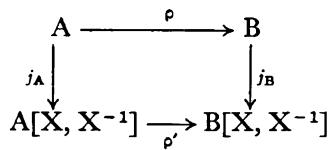
\includegraphics[keepaspectratio]{images/part002_18d5f867.jpg}}

（其中 \(\rho\) 是定义 B 上 A-代数结构的同态，\(\rho'\) 是由它典范导出的同态）是交换的，这由定义 (5) 立即验证。设 \(x\) 是 B 中在 A 上整的元素；则 \(j_{\mathrm{B}}(x)\) 在 \(\mathbf{A}[\mathbf{X}, \mathbf{X}^{-1}]\) 上是整的（第 1 节，命题 2），因此由第 5 节命题 16 可知，存在整数 \(m > 0\) 使得 \(\mathbf{X}^m j_{\mathrm{B}}(x)\) 是 \(\mathbf{B}[\mathbf{X}]\) 中在 \(\mathbf{A}[\mathbf{X}]\) 上整的元素。再由第 3 节命题 12 推出多项式 \(\mathbf{X}^m j_{\mathrm{B}}(x)\) 的系数在 A 上是整的；由于这些系数按定义就是 \(x\) 的齐次分量，可见它们都在 A 上是整的，这就证明了 \(\mathbf{A}'\) 是 B 的分次子代数。

现在设 \(x \in \mathbf{A}_i'\) ，其中 \(i < 0\) ；本节开头的注表明 \(x\) 满足形如 (4) 的方程，其中 \(a_k' \in \mathbf{A}_{ki}\) （\(1 \leqslant k \leqslant n\)）。若 \(\mathbf{A}_j = 0\) （\(j < 0\)），则 \(x^n = 0\) ；又若 \(B\) 是约化环，则可断定 \(x = 0\) ，从而在此情形 \(\mathbf{A}_i' = 0\) （对所有 \(i < 0\)）。

回忆（第 II 章，§ 2，第 9 节）：若 \(\mathbf{A} = \bigoplus_{i\in \mathbf{Z}}\mathbf{A}_i\) 是分次环，S 是由齐次元组成的 A 的乘性子集，则在 \(\mathrm{S}^{-1}\mathrm{A}\) 上可定义一个分次环结构，只需把集 \((\mathrm{S}^{-1}\mathrm{A})_i\) （\(i\) 次齐次元组成的集）取作形如 \(a / s\) 的元素组成的集，其中 \(a\in \mathbf{A}\) 与 \(s\in \mathbf{S}\) 是齐次的，且 \(\deg (a) - \deg (s) = i\) 。

引理 4. 设 \(\mathbf{A} = \bigoplus_{i\in \mathbf{Z}}\mathbf{A}_i\) 是分次整环，S 是 A 的 \(\neq 0\) 齐次元组成的集。

\begin{enumerate}
\def\labelenumi{(\roman{enumi})}
\item
  每个 \(\neq 0\) 的齐次元（\(\mathbf{S}^{-1}\mathbf{A}\) 中的）都是可逆的，环 \(\mathbf{K}_0 = (\mathbf{S}^{-1}\mathbf{A})_0\) 是域，且诸 \(i\in \mathbf{Z}\) 中使 \((\mathrm{S}^{-1}\mathrm{A})_i\neq 0\) 者组成的集是子群 \(q\mathbf{Z}\) ——\(\mathbf{Z}\) 的子群（其中 \(q\geqslant 0\) ）。
\item
  假设 \(q \geqslant 1\) ，并设 \(t\) 是 \((\mathbf{S}^{-1}\mathbf{A})_q\) 的非零元素。则 \(\mathbf{K}_0\) -同态 \(f\) （它把多项式环 \(\mathbf{K}_0[\mathbf{X}]\) 映到 \(\mathbf{S}^{-1}\mathbf{A}\) ，把 \(\mathbf{X}\) 映到 \(t\) ）可扩张为 \(\mathbf{K}_0[\mathbf{X}, \mathbf{X}^{-1}]\) 到 \(\mathbf{S}^{-1}\mathbf{A}\) 上的同构，且 \(\mathbf{S}^{-1}\mathbf{A}\) 是整闭的。
\end{enumerate}

(i) 中的断言由诸定义及 A 是整环这一假设立即得出，因为若 \(a/s\) 与 \(a'/s'\) 是两个 \(\neq 0\) 齐次元，属于 \(\mathrm{S}^{-1}\mathrm{A}\) ，次数分别为 \(i\) 与 \(i'\) ，则 \(aa'/ss'\) 是 \(\neq 0\) 齐次元，且次数为 \(i+i'\) 。为证 (ii)，注意由于 \(t\) 在 \(\mathrm{S}^{-1}\mathrm{A}\) 中可逆，同态 \(f\) 以唯一方式扩张为同态 \(\bar{f}: \mathrm{K}_0[\mathrm{X}, \mathrm{X}^{-1}] \to \mathrm{S}^{-1}\mathrm{A}\) ，且必有 \(\bar{f}(\mathrm{X}^{-1}) = t^{-1}\) 。另一方面，由 \(q\) 的定义，每个 \(\neq 0\) 齐次元（\(\mathrm{S}^{-1}\mathrm{A}\) 中的）的次数都形如 \(qn\)（ \(n \in \mathbf{Z}\) ），从而可唯一地写成 \(\lambda t^n\) 的形式，其中 \(\lambda \in \mathrm{K}_0\) （因为 \(\mathrm{S}^{-1}\mathrm{A}\) 是整环）；因此 \(\bar{f}\) 是双射。最后，我们知道 \(\mathrm{K}_0[\mathrm{X}]\) 是整闭的（第 3 节，命题 10），从而 \(\mathrm{K}_0[\mathrm{X}, \mathrm{X}^{-1}]\) 也是整闭的（第 5 节，命题 16 的推论 1），这就完成了引理的证明。

命题 21. 设 \(\mathbf{A} = \bigoplus_{i\in \mathbf{Z}}\mathbf{A}_i\) 是分次整环，S 是 A 的 \(\neq 0\) 齐次元组成的集。则 A 的整闭包 \(\mathbf{A}'\) 是 \(\mathbf{S}^{-1}\mathbf{A}\) 的分次子环。若进一步 \(\mathbf{A}_i = 0\) （\(i < 0\)），则 \(\mathbf{A}_i' = 0\) （\(i < 0\)）。

若 \(A = A_{0}\) ，命题是平凡的。否则可应用引理 4；环 \(S^{-1}A\) 是整闭整环，因此 \(A' \subset S^{-1}A\) ；由于 \(S^{-1}A\) 是分次的，由命题 20，\(A'\) 也是分次的；后一断言同样由命题 20 得出。

推论 1. 在命题 21 的假设与记号下，若 \(\mathbf{S}^{-1}\mathbf{A}\) 中在 \(\mathbf{A}\) 上是整的每个齐次元都属于 \(\mathbf{A}\) ，则 \(\mathbf{A}\) 是整闭的。

则 \(\mathbf{A}_i' \subset \mathbf{A}\) 对所有 \(i \in \mathbf{Z}\) 成立，从而 \(\mathbf{A}' = \mathbf{A}\) 。

推论 2. 若 \(\mathbf{A} = \bigoplus_{i\in \mathbf{Z}}\mathbf{A}_i\) 是整闭的分次整环，则整环 \(\mathbf{A}_0\) 是整闭的。

\(\mathbf{K}_0\) （\(\mathbf{A}_0\) 的分式域，按命题 21 的记号）被等同于

\(S^{-1}A\) 的由 0 次齐次元组成的环的一个子环；因此，\(K_{0}\) 中在 \(A_{0}\) 上（更不必说在 A 上）是整的每个元素按假设都属于 \(A_{0}\) 。

推论 3. 设 \(\mathbf{A} = \bigoplus_{i\in \mathbf{Z}}\mathbf{A}_i\) 是整闭的分次整环。则对每个整数 \(d > 0\) ，环 \(\mathbf{A}^{(d)}\) （第 III 章，§1，第 3 节）是整闭整环。

设 U 是由 \(\neq0\) 齐次元（\(A^{(d)}\) 中的）组成的集，并设 x 是 \(U^{-1}A^{(d)}\) 的在 \(A^{(d)}\) 上因而在 A 上是整的齐次元；由于 \(x\in S^{-1}A\) ，按假设 x 属于 A；由于其次数被 d 整除，它属于 \(A^{(d)}\) ，于是由推论 1 即得 \(A^{(d)}\) 是整闭的。

\subsection{应用：代数的自同构群的不变量}

给定环 K、K-代数 A 和群 G，若满足：(1) 集 A 以 G 为算子群（《代数》，第 I 章，§ 7，第 2 节）；(2) 对所有 \(\sigma \in G\) ，映射 \(x \mapsto \sigma \cdot x\) 是 K-代数 A 的自同态（且由于它是双射（同前），因而是自同构），则我们说 G 作用于 A。我们将以 \(A^{G}\) 表示 A 中在 G 下不变的元素组成的集；显然它是 A 的子 K-代数。

若 \(\mathcal{G}\) 在 A 中的每条轨道（《代数》，第 I 章，第 IV 分册勘误）都是有限的，则我们说 \(\mathcal{G}\) 是 A 上局部有限的算子群。

命题 22. 设 A 是（交换）K-代数，G 是 A 上局部有限的算子群。则 A 在子代数 \(\mathbf{A}^{\mathcal{G}}\) 上是整的。

对所有 \(x \in \mathbf{A}\) ，设 \(x_{i} (1 \leqslant i \leqslant n)\) 是 \(x\) 在 \(\mathcal{G}\) 下轨道中的不同元素；对所有 \(\sigma \in \mathcal{G}\) ，存在置换 \(\pi_{\sigma}\) （集 \(\{1, 2, \ldots, n\}\) 的置换），使得 \(\sigma. x_{i} = x_{\pi_{\sigma}(i)}\) （\(1 \leqslant i \leqslant n\)）；因此 \(x_{i}\) 的初等对称函数是 \(\mathbf{A}\) 中在 \(\mathcal{G}\) 下不变的元素，换言

之，是 \(\mathbf{A}^{\mathcal{G}}\) 的元素。由于 \(x\) 是首一多项式 \(\prod_{i=1}^{n} (\mathbf{X} - x_i)\) 的根，且该多项式的系数属于 \(\mathbf{A}^{\mathcal{G}}\) ，故 \(x\) 在 \(\mathbf{A}^{\mathcal{G}}\) 上是整的。

定理 2. 设 A 是有限生成的 K-代数，G 是 A 上局部有限的算子群。则 A 是有限生成的 \(\mathbf{A}^{\mathcal{G}}\)-模；若进一步 K 是 Noether 环，则 \(A^{G}\) 是有限生成的 K-代数。

设 \((a_{j})_{1\leqslant j\leqslant m}\) 是 K-代数 A 的生成系；由于更不必说 \(\mathbf{A} = \mathbf{A}^{\mathcal{G}}[a_1,\ldots ,a_m]\) ，且由命题 22 诸 \(a_{j}\) 在 \(\mathbf{A}^{\mathcal{G}}\) 上是整的，故第一个断言由第 1 节命题 4 得出。第二个断言是下述引理的推论：

引理 5. 设 K 是 Noether 环，B 是有限生成的 K-代数，C 是 B 的子 K-代数且 B 在 C 上是整的。则 C 是有限生成的 K-代数。

设 \((x_{i})_{1\leqslant i\leqslant n}\) 是 K-代数 B 的有限生成系。对所有 \(i\) ，按假设存在首一多项式 \(\mathbf{P}_i\in \mathbf{C}[\mathbf{X}]\) 使得 \(\mathrm{P_i}(x_i) = 0\) 。设 \(\mathbf{C}'\) 是由诸 \(\mathbf{P}_i\) （ \(1\leqslant i\leqslant n\) ）的系数生成的 C 的子 K-代数；显然诸 \(x_{i}\) 在 \(\mathbf{C}'\) 上是整的，且 \(\mathbf{B} = \mathbf{C}'[x_1,\dots,x_n]\) ；因此 B 是有限生成的 \(\mathbf{C}'\) -模（第 1 节，命题 4）。另一方面，\(\mathbf{C}'\) 是 Noether 环（第 III 章，§2，第 10 节，定理 2 的推论 3）；因此 C 是有限生成的 \(\mathbf{C}'\) -模，这就证明了 C 是有限生成的 K-代数。

注. 由所有 \(\sigma \in \mathcal{G}\) （满足 \(\sigma a_{j} = a_{j}\) ，\(1 \leqslant j \leqslant m\) ）组成的集显然使 A 的每个元素不变。因此，使 A 的每个元素都不变的正规子群 \(\mathcal{H}\) （\(\mathcal{G}\) 的）在 \(\mathcal{G}\) 中的指数有限，从而可以把 A 看作以有限群 \(\mathcal{G}/\mathcal{H}\) 为算子群；显然 \(\mathrm{A}^{\mathcal{G}/\mathcal{H}} = \mathrm{A}^{\mathcal{G}}\) 。

设 S 是环 A 的乘性子集，G 是作用于 A 且使 S 稳定的群；则对所有 \(\sigma\in G\) ，存在唯一的自同态 \(z\mapsto\sigma.z\) （环 \(S^{-1}A\) 的），使得 \(\sigma.(a/1)=(\sigma.a)/1\) （对所有 \(a\in A\)）；它由公式 \(\sigma.(a/s)=(\sigma.a)/( \sigma.s)\) 给出，其中 \(a\in A\) ，\(s\in S\) （第 II 章，§2，第 1 节，命题 2）；若 \(\tau\) 是 G 的另一个元素，则显然 \(\sigma.(\tau.z)=(\sigma\tau).z\) 对所有 \(z\in S^{-1}A\) 成立，因而群 G 作用于环 \(S^{-1}A\) 。

命题 23. 设 A 是 K-代数，\(\mathcal{G}\) 是 A 上局部有限的算子群，S 是 A 的在 \(\mathcal{G}\) 下稳定的乘性子集，\(\mathrm{S}^{\mathcal{G}}\) 是集 \(\mathrm{S} \cap \mathrm{A}^{\mathcal{G}}\) 。则从 \((\mathrm{S}^{\mathcal{G}})^{-1}\mathrm{A}\) 到 \(\mathrm{S}^{-1}\mathrm{A}\) 的典范映射（第 II 章，§ 2，第 1 节，命题 2 的推论 2）是同构，且它把 \((\mathrm{S}^{\mathcal{G}})^{-1}\mathrm{A}^{\mathcal{G}}\) 映到 \((\mathrm{S}^{-1}\mathrm{A})^{\mathcal{G}}\) 。

对所有 \(s \in S\) ，设 \(s, s_1, \ldots, s_q\) 是 \(s\) 在 \(\mathcal{G}\) 下轨道中的不同元素；由于 \(ss_1 \ldots s_q \in S^{\mathcal{G}}\) ，第一个断言由第 II 章，§ 2，第 3 节，命题 8 得出。把 \((S^{\mathcal{G}})^{-1}A\) 与 \(S^{-1}A\) 典范地等同起来，则显然 \((S^{\mathcal{G}})^{-1}A^{\mathcal{G}}\) 的每个元素都在 \(\mathcal{G}\) 下不变。反之，设 \(a/t\) 是 \((S^{\mathcal{G}})^{-1}A\) 中在 \(\mathcal{G}\) 下不变的元素（ \(a \in A\) ，\(t \in S^{\mathcal{G}}\) ）；若 \(a_j\) （ \(1 \leqslant j \leqslant m\) ）是 \(a\) 在 \(\mathcal{G}\) 下轨道中的不同元素，则 \(a_j/t = a/t\) （\(1 \leqslant j \leqslant m\)），因此存在 \(s \in S^{\mathcal{G}}\) 使得 \(s(a_j - a) = 0\) （\(1 \leqslant j \leqslant m\)）；换言之，\(sa\) 在 \(\mathcal{G}\) 下不变，且由于 \(a/t = (sa)/(st)\) ，当然有 \(a/t \in (S^{\mathcal{G}})^{-1}A^{\mathcal{G}}\) 。

推论. 设 A 是整环，K 是其分式域，G 是 A 上局部有限的算子群。则 G 作用于 K，且 \(K^{G}\) 是 \(A^{G}\) 的分式域。

A - \{0\} 在 G 下稳定。

\section{素理想的提升}

\subsection{第一存在定理}

定义 1. 设 A、A' 是两个环，h: A → A' 是环同态。若 \iffalse h\^{}\{-1\}(a')\fi\(a = h^{-1}(a')\)，则称 A' 的理想 a' 位于 A 的理想 a 之上。

因此，说素理想 \(\mathfrak{p}'\) （\(\mathbf{A}'\) 的）位于理想 \(\mathfrak{p}\) （\(\mathbf{A}\) 的）之上，就是指 \(\mathfrak{p}\) 是 \(\mathfrak{p}'\) 在连续映射 \(^a h\) ： \(\operatorname{Spec}(\mathbf{A}') \to \operatorname{Spec}(\mathbf{A})\) （它与 \(h\) 相伴）下的像（第 II 章，§ 4，第 3 节）。

注意，为使 \(\mathbf{A}'\) 中存在位于 \(\mathbf{A}\) 的理想 (0) 之上的理想，必须而且只需 \(h: \mathbf{A} \to \mathbf{A}'\) 是单射。

设 \(\mathfrak{a}\) 是 \(\mathbf{A}\) 的理想；对 \(h\) 取商，得到同态 \(h_1: \mathbf{A} / \mathfrak{a} \to \mathbf{A}' / \mathfrak{a}'\) ；说 \(\mathfrak{a}'\) 是 \(\mathbf{A}'\) 的位于 \(\mathfrak{a}\) 之上的理想，等价于说 \(\mathfrak{a}\mathbf{A}' \subset \mathfrak{a}'\) 且 \(\mathfrak{a}' / \mathfrak{a}\mathbf{A}'\) 是 \(\mathbf{A}' / \mathfrak{a}\mathbf{A}'\) 的位于 (0) 之上的理想。

引理 1. 设 \(h: \mathbf{A} \to \mathbf{A}'\) 是环同态，\(\mathbf{S}\) 是 \(\mathbf{A}\) 的乘性子集，\(i = i_{\mathbf{A}}^{\mathbf{S}}: \mathbf{A} \to \mathbf{S}^{-1}\mathbf{A}\) ，\(i' = i_{\mathbf{A}'}^{h(\mathbf{S})}: \mathbf{A}' \to \mathbf{S}^{-1}\mathbf{A}' = (h(\mathbf{S}))^{-1}\mathbf{A}'\) 是典范同态，而 \(h_1 = \mathbf{S}^{-1}h: \mathbf{S}^{-1}\mathbf{A} \to \mathbf{S}^{-1}\mathbf{A}'\) ，于是有交换图

\pandocbounded{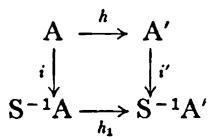
\includegraphics[keepaspectratio]{images/part002_a0a90333.jpg}}

设 \(\mathfrak{p}\) 是 \(\mathbf{A}\) 的素理想且 \(\mathfrak{p} \cap \mathbf{S} = \varnothing\) 。则 \(\mathfrak{a}' \mapsto \mathbf{S}^{-1}\mathfrak{a}'\) 是从集 \(\mathcal{F}\) ——\(\mathbf{A}'\) 的位于 \(\mathfrak{p}\) 之上的理想组成的集——到集 \(\mathcal{F}_1\) ——\(\mathbf{S}^{-1}\mathbf{A}'\) 的位于 \(\mathbf{S}^{-1}\mathfrak{p}\) 之上的理想组成的集——上的满射，而映射 \(\mathfrak{a}_1' \mapsto i'^{-1}(\mathfrak{a}_1')\) 是 \(\mathcal{F}_1\) 到 \(\mathcal{F}\) 中关于 \(h(S)\) 饱和的理想组成的集上的双射；特别地，\(\mathfrak{p}' \mapsto \mathbf{S}^{-1}\mathfrak{p}'\) 是从 \(\mathbf{A}'\) 的位于 \(\mathfrak{p}\) 之上的素理想组成的集到 \(\mathbf{S}^{-1}\mathbf{A}'\) 的位于 \(\mathbf{S}^{-1}\mathfrak{p}\) 之上的素理想组成的集上的双射。

我们知道 \(\mathbf{S}^{-1}\mathfrak{p}\) 是 \(\mathbf{S}^{-1}\mathbf{A}\) 的素理想，且 \(i^{-1}(\mathbf{S}^{-1}\mathfrak{p}) = \mathfrak{p}\) （第 II 章，§ 2，第 5 节，命题 11）；若存在理想 \(\mathfrak{b}'\) （\(\mathbf{S}^{-1}\mathbf{A}'\) 的位于 \(\mathbf{S}^{-1}\mathfrak{p}\) 之上的理想），则 \(h(i'^{-1}(\mathfrak{b}')) = i^{-1}(h_1(\mathfrak{b}')) = \mathfrak{p}\) ；由于 \(\mathbf{S}^{-1}.i'^{-1}(\mathfrak{b}') = \mathfrak{b}'\) （同前），这已经表明 \(\mathcal{F}\) 在映射 \(\mathfrak{a}'\mapsto\mathrm{S}^{-1}\mathfrak{a}'\) 下的像包含 \(\mathcal{F}_{1}\) 。另一方面，若 \(\mathfrak{a}'\in\mathcal{F}\) ，\(a\in\mathbf{A}\) 且 \(s\in\mathbf{S}\) ，则有下列等价关系

\[
\begin{array}{l} h _ {1} (a / s) \in \mathrm{S} ^ {- 1} \mathfrak {a} ^ {\prime} \Leftrightarrow h (a) / h (s) \in \mathrm{S} ^ {- 1} \mathfrak {a} ^ {\prime} \\ \Leftrightarrow \text { there   exists } t \in \mathrm{S} \text { such   that } h (t) h (a) \in \mathfrak {a} ^ {\prime} \\ \Leftrightarrow \text { there   exists } t \in \mathrm{S} \text { such   that } t a \in \mathfrak {p} \\ \Leftrightarrow a / s \in \mathrm{S} ^ {- 1} \mathfrak {p}. \end{array}
\]

于是 \(h_1^{-1}(\mathbf{S}^{-1}\mathfrak{a}') = \mathbf{S}^{-1}\mathfrak{p}\) ，这就完成了 \(\mathcal{F}\) 在映射 \(\mathfrak{a}' \mapsto \mathbf{S}^{-1}\mathfrak{a}'\) 下的像等于 \(\mathcal{F}_1\) 的证明；其余断言由第 II 章，§ 2，第 5 节，命题 11 得出。

命题 1. 设 \(h: \mathbf{A} \to \mathbf{A}'\) 是环同态且 \(\mathbf{A}'\) 在 \(\mathbf{A}\) 上是整的，\(\mathfrak{p}'\) 是 \(\mathbf{A}'\) 的素理想，而 \(\mathfrak{p} = h^{-1}(\mathfrak{p}')\) 。为使 \(\mathfrak{p}\) 极大，必须而且只需 \(\mathfrak{p}'\) 极大。

记 \(\mathrm{B} = \mathrm{A} / \mathfrak{p}\) ，\(\mathrm{B}' = \mathrm{A}' / \mathfrak{p}'\) ，并设 \(h_1 \colon \mathrm{B} \to \mathrm{B}'\) 是对 \(h\) 取商得到的同态；\(\mathrm{B}\) 与 \(\mathrm{B}'\) 是整环，且 \(\mathrm{B}'\) 在 \(\mathrm{B}\) 上是整的（§ 1，第 1 节，命题 2）。说 \(\mathfrak{p}\) （相应地 \(\mathfrak{p}'\) ）极大，就是指 \(\mathrm{B}\) （相应地 \(\mathrm{B}'\) ）是域。于是命题由下述引理得出：

引理 2. 设 B 是整环，A 是 B 的子环且 B 在 A 上是整的。为使 B 是域，必须而且只需 A 是域。

若 A 是域，则对 B 中所有 \(y \neq 0\) ，A[y] 按假设（ \(\S 1\) ，定理 1）是有限生成的 A-模；由于 A[y] 是整环，它是域（《代数》，第 V 章，\(\S 2\) ，第 1 节，命题 1），更不必说 y 在 B 中可逆，因而 B 是域。反之，设 B 是域，并设 A 中 \(z \neq 0\) ；由于 \(z^{-1} \in B\) ，\(z^{-1}\) 在 A 上是整的，换言之存在整依赖方程

\[
z ^ {- n} + a _ {1} z ^ {- (n - 1)} + \dots + a _ {n} = 0
\]

其中 \(a_{i} \in \mathbf{A}\) ；而这关系式表明

\[
- z ^ {- 1} = a _ {1} + a _ {2} z + \dots + a _ {n} z ^ {n - 1} \in A,
\]

因而 A 当然是域。

推论 1. 设 \(h: \mathbf{A} \to \mathbf{A}'\) 是环同态且 \(\mathbf{A}'\) 在 \(\mathbf{A}\) 上是整的，\(\mathfrak{p}\) 是 \(\mathbf{A}\) 的素理想，\(\mathfrak{p}'\) 与 \(\mathfrak{a}'\) 是 \(\mathbf{A}'\) 的位于 \(\mathfrak{p}\) 之上且满足 \(\mathfrak{p}' \subset \mathfrak{a}'\) 的两个理想。若 \(\mathfrak{p}'\) 是素理想，则 \(\mathfrak{a}' = \mathfrak{p}'\) 。

记 \(S = A - p\) ；则 \(S^{-1}A'\) 在 \(S^{-1}A\) 上是整的（§ 1，第 5 节，命

题 16），\(S^{-1}p\) 是 \(S^{-1}A\) 的极大理想（第 II 章，§2，第 5 节，命题 11），\(S^{-1}a'\) 与 \(S^{-1}p'\) 是 \(S^{-1}A'\) 的位于 \(S^{-1}p\) 之上的理想（引理 1），且 \(S^{-1}a' \supseteq S^{-1}p'\) 。由于 \(S^{-1}p'\) 是素理想，由命题 1 它是极大的，因而 \(S^{-1}p' = S^{-1}a'\) ；于是 \(a'\) 包含在 \(p'\) 关于 \(h(S)\) 的饱和中，而后者等于 \(p'\) （第 II 章，§2，第 5 节，命题 11）。

推论 2. 设 A' 是整环，A 是 A' 的子环且 A' 在 A 上是整的，f 是从 A' 到环 B 的同态。若 f 在 A 上的限制是单射，则 f 是单射。

若 \(a'\) 是 f 的核，则假设是指 \(a' \cap A = (0)\) ；由于 \(A'\) 是整环，可应用推论 1，取 p 与 \(p'\) 分别为 A 的理想 (0) 与 \(A'\) 的理想 (0)，由此得 \(a' = (0)\) 。

推论 3. 设 \(h: \mathbf{A} \to \mathbf{A}'\) 是环同态且 \(\mathbf{A}'\) 在 \(\mathbf{A}\) 上是整的，\(\mathfrak{m}\) 是 \(\mathbf{A}\) 的极大理想，并设 \(\mathbf{A}'\) 中只有有限个不同的极大理想 \(\mathfrak{m}_j' (1 \leqslant j \leqslant n)\) 位于 \(\mathfrak{m}\) 之上。设 \(\mathfrak{q}_j'\) 是 \(\mathfrak{mA}'\) 关于 \(\mathfrak{m}_j'\) 的饱和（第 II 章，§ 2，第 4 节）。则：

\begin{enumerate}
\def\labelenumi{(\roman{enumi})}
\item
  在环 \(\mathbf{A}' / \mathfrak{q}_j'\) 中，零因子是 \(\mathfrak{m}_j' / \mathfrak{q}_j'\) 的元素，且它们都是幂零的（ \(1 \leqslant j \leqslant n\) ）。
\item
  \(mA' = \bigcap_{j} q_{j}' = \prod_{j} q_{j}'\) .
\item
  典范同态 \(\mathbf{A}' / \mathfrak{m}\mathbf{A}' \to \prod_j (\mathbf{A}' / \mathfrak{q}_j')\) 是双射。
\end{enumerate}

为使 A' 的素理想包含 mA'，必须而且只需它在 h 下的原像包含 m，从而它位于 m 之上，因为 m 在 A 中是极大的；于是诸 \(m_{j}'\) 是 A' 的包含 mA' 的仅有素理想（命题 1），因此 \(r' = \bigcap_{j} m_{j}'\) 是 mA' 的根（第 II 章，§2，第 6 节，命题 13 的推论 1）。按 \(q_{j}'\) 的定义，模 \(q_{j}'\) 的类（\(\mathbf{A}' - \mathfrak{m}_{j}'\) 中元素的）不是 \(A'/q_{j}'\) 中的零因子；另一方面，由于诸 \(m_{j}'\) 是互不相同的极大理想，对每个指标 j，存在元素 \(a_{j}'\) ，它属于 \(\bigcap_{i \neq j} m_{i}'\) 而不属于 \(m_{j}'\) （第 II 章，§1，第 1 节，命题 4）；于是对所有 \(x \in m_{j}'\) ，有 \(a_{j}'x \in r'\) ，因而模 \(q_{j}'\) 之下 \(a_{j}'x\) 的类是幂零的，又由于 \(a_{j}'\) 的类不是零因子，可断定 x 的类是幂零的；换言之，\(m_{j}'\) 是 \(q_{j}'\) 的根，这就证明了 (i)。由此可得诸 \(q_{j}'\) 两两互素（第 II 章，§1，第 1 节，命题 3）；因此，考虑到第 II 章，§1，第 2 节，命题 5，(iii) 将是 (ii) 的推论。为证 (ii)，注意在环 A'/mA' 中，诸 \(m_{j}'/mA'\) 是仅有的极大理想，而 \(q_{j}'/mA'\) 是 (0) 关于 \(m_{j}'/mA'\) 的饱和（第 II 章，§2，第 4 节）；于是只需考察 mA' = (0) 的情形；此时 (ii) 的断言由第 II 章，§3，第 3 节，定理 1 的推论 2 得出。

注 (1) 若 \(\mathbf{A}'\) 是 Noether 环，则由 (i) 与 (ii) 可得 \((\mathfrak{q}_j')_{1 \leqslant j \leqslant n}\) 是 \(\mathfrak{mA}'\) 的唯一准素分解（第 IV 章，§ 2，第 3 节）。

定理 1. 设 \(h: \mathbf{A} \to \mathbf{A}'\) 是单环同态且 \(\mathbf{A}'\) 在 \(\mathbf{A}\) 上是整的，\(\mathfrak{p}\) 是 \(\mathbf{A}\) 的素理想。则存在素理想 \(\mathfrak{p}'\) （\(\mathbf{A}'\) 的），位于 \(\mathfrak{p}\) 之上。

先设 A 是局部环，p 是 A 的极大理想；则对每个极大理想 \(m'\) （\(A'\) 的），\(\bar{h}^{-1}(m')\) 是 A 的极大理想（命题 1），因而等于 p，这就证明了定理在此情形成立（因为按假设 \(A'\) 包含 A，从而不约化为 0）。一般情形下，记 \(S = A - p\) ；则 \(S^{-1}A\) 是局部环，其极大理想为 \(S^{-1}p\) （第 II 章，§2，第 5 节，命题 11），\(S^{-1}h: S^{-1}A \to S^{-1}A'\) 是单射（第 II 章，§2，第 4 节，定理 1），且 \(S^{-1}A'\) 在 \(S^{-1}A\) 上是整的（§1，第 5 节，命题 16）；于是存在素理想 \(q'\) （\(S^{-1}A'\) 的），位于 \(S^{-1}p\) 之上，且我们知道 \(q' = S^{-1}p'\) ，其中 \(p'\) 是 \(A'\) 的位于 p 之上的素理想（引理 1）。

若 \(h: \mathbf{A} \to \mathbf{A}'\) 不是单射，定理 1 便未必成立，同态 \(\mathbf{Z} \to \mathbf{Z}/n\mathbf{Z}\) （ \(n > 1\) ）的例子即表明这一点。但定理 1 可应用于典范单射 \(h(\mathbf{A}) \to \mathbf{A}'\) ；换言之，定理 1 的结论对素理想 \(\mathfrak{p}\) （它包含 \(\operatorname{Ker}(h)\) ）成立。

推论 1. 在定理 1 的假设与记号下，\(h^{-1}(pA') = p\) 。

\(\mathfrak{pA}' \subset \mathfrak{p}'\) 且 \(\overline{h}(\mathfrak{p}') = \mathfrak{p}\) 。

推论 2. 设 \(h: \mathbf{A} \to \mathbf{A}'\) 是环同态且 \(\mathbf{A}'\) 在 \(\mathbf{A}\) 上是整的，\(\mathfrak{a}\) 与 \(\mathfrak{p}\) 是 \(\mathbf{A}\) 的满足 \(\mathfrak{a} \subset \mathfrak{p}\) 的两个理想，\(\mathfrak{a}'\) 是 \(\mathbf{A}'\) 的位于 \(\mathfrak{a}\) 之上的理想。设 \(\mathfrak{p}\) 是素理想。则存在素理想 \(\mathfrak{p}'\) （\(\mathbf{A}'\) 的），位于 \(\mathfrak{p}\) 之上且包含 \(\mathfrak{a}'\) 。

若 \(h_1 \colon \mathbf{A} / \mathfrak{a} \to \mathbf{A}' / \mathfrak{a}'\) 是对 \(h\) 取商得到的同态，则 \(h_1\) 按假设是单射，且 \(\mathbf{A}' / \mathfrak{a}'\) 在 \(\mathbf{A} / \mathfrak{a}\) 上是整的（§ 1，第 1 节，命题 2）；于是存在素理想 \(\mathfrak{p}' / \mathfrak{a}'\) （\(\mathbf{A}' / \mathfrak{a}'\) 中的； \(\mathfrak{p}'\) 在 \(\mathbf{A}'\) 中为素），位于 \(\mathfrak{p} / \mathfrak{a}\) 之上（定理 1），而 \(\mathfrak{p}'\) 就是所求的理想。

推论 3. 设 A 是环，A' 是包含 A 且在 A 上是整的环。若 R' 是 A' 的 Jacobson 根，则 R' ∩ A 是 A 的 Jacobson 根。

设 \(\mathfrak{R}\) 是 A 的 Jacobson 根。对每个极大理想 \(\mathfrak{m}'\) （\(\mathbf{A}'\) 的），\(\mathfrak{m}' \cap \mathbf{A}\) 是 A 的极大理想（命题 1），因而 \(\mathfrak{R} \subset \mathfrak{m}' \cap \mathbf{A}\) ，从而 \(\mathfrak{R} \subset \mathfrak{R}' \cap \mathbf{A}\) （《代数》，第 VIII 章，§ 5，第 3 节，定义 3）。反之，设 \(x \in \mathfrak{R}' \cap \mathbf{A}\) ；对 A 的每个极大理想 \(\mathfrak{m}\) ，\(\mathbf{A}'\) 中存在位于 \(\mathfrak{m}\) 之上的素理想（定理 1），且该理想 \(\mathfrak{m}'\) 必为极大的（命题 1），因而 \(x \in \mathfrak{m}' \cap \mathbf{A} = \mathfrak{m}\) ，从而 \(x \in \mathfrak{R}\) 。

推论 4. 设 A 是环，A' 是包含 A 且在 A 上是整的环，f 是从 A 到代数闭域 L 的同态。则 f 可扩张为从 A' 到 L 的同态。

设 p 是 f 的核，由于 \(f(\mathbf{A}) \subset \mathbf{L}\) 是整环，它是素理想；设 \(p'\) 是 \(A'\) 的位于 p 之上的素理想（定理 1）。则 A/p 典范地等同于 \(A'/p'\) 的一个子环，且 \(A'/p'\) 在 A/p 上是整的（§ 1，第 1 节，命题 2）。同态 f 取商后定义了 A/p 到 L 的子环 \(f(\mathbf{A})\) 上的同构，而该同构可扩张为 A/p 的分式域 K 到 L 的一个子域上的同构 g。由于 \(K'\) （\(A'/p'\) 的分式域）在 K 上是代数的，g 可扩张为一个同构 \(g'\) （从 \(K'\) 到 L 的一个子域上的）（《代数》，第 V 章，§ 4，第 2 节，定理 1 的推论）；若 \(\pi': A' \to A'/p'\) 是典范同态，则 \(g' \circ \pi'\) 是从 \(A'\) 到 L 的扩张 f 的同态。

注 (2). 设 \(h \colon \mathbf{A} \to \mathbf{A}'\) 是环同态且 \(\mathbf{A}'\) 在 \(\mathbf{A}\) 上是整的；则相伴的连续映射 \(^a h \colon \operatorname{Spec}(\mathbf{A}') \to \operatorname{Spec}(\mathbf{A})\) 是闭的。对每个理想 \(\mathfrak{a}'\) （\(\mathbf{A}'\) 的），\(\mathbf{A}' / \mathfrak{a}'\) 在 \(\mathbf{A}'\) 上因而在 \(\mathbf{A}\) 上是整的（§ 1，第 1 节，命题 6），且 \(\operatorname{Spec}(\mathbf{A}' / \mathfrak{a}')\) 等同于闭子空间 \(\mathbf{V}(\mathfrak{a}')\) （\(\operatorname{Spec}(\mathbf{A}')\) 的）；为证 \(^a h\) 是闭的，于是（把 \(\mathbf{A}'\) 换成 \(\mathbf{A}' / \mathfrak{a}'\) ）只需证明 \(\operatorname{Spec}(\mathbf{A}')\) 在 \(^a h\) 下的像是 \(\operatorname{Spec}(\mathbf{A})\) 的闭子集即可；而由定理 1，这个像正是 \(\mathbf{A}\) 的包含理想 \(\operatorname{Ker}(h)\) 的素理想组成的集，且由 \(\operatorname{Spec}(\mathbf{A})\) 上拓扑的定义，这个集是闭的。

命题 2. 设 \(h: \mathbf{A} \to \mathbf{A}'\) 是环同态且 \(\mathbf{A}'\) 在 \(\mathbf{A}\) 上是整的，\(\mathfrak{p}\) 是 \(\mathbf{A}\) 的素理想，\(S = A - \mathfrak{p}\) ，\((\mathfrak{p}_i')_{i \in I}\) 是 \(\mathbf{A}'\) 的位于 \(\mathfrak{p}\) 之上的全部素理想组成的族，而 \(S' = \bigcap_{i \in I} (\mathbf{A}' - \mathfrak{p}_i')\) ；则 \(S^{-1}A' = S'^{-1}A'\) 。

事实上，按定义 \(h(\mathbf{S}) \subset \mathbf{S}'\) ，且由于

\[
h (\mathbf {S}) ^ {- 1} \mathbf {A} ^ {\prime} = \mathbf {S} ^ {- 1} \mathbf {A} ^ {\prime},
\]

根据第 II 章，§ 2，第 3 节，命题 8，只需证明：若素理想 \(\mathfrak{q}'\) （\(\mathbf{A}'\) 的）不与 \(h(\mathbf{S})\) 相交，则它也不与 \(\mathbf{S}'\) 相交。现设 \(\mathfrak{q}' \cap h(\mathbf{S}) = \varnothing\) ，并令 \(\mathfrak{q} = \bar{h}^{-1}(\mathfrak{q}')\) ；则 \(\mathfrak{q} \cap \mathbf{S} = \varnothing\) ，换言之 \(\mathfrak{q} \subset \mathfrak{p}\) 。由于按定义 \(\mathfrak{q}'\) 位于 \(\mathfrak{q}\) 之上，由命题 1 的推论 2，存在指标 \(\iota\) 使得 \(\mathfrak{q}' \subset \mathfrak{p}_i'\) ，因而 \(\mathfrak{q}' \cap \mathbf{S}' = \varnothing\) ，这就完成了证明。

命题 3. 设 \(h: \mathbf{A} \to \mathbf{A}'\) 是环同态且 \(\mathbf{A}'\) 是有限生成的 A-模；则对每个素理想 \(\mathfrak{p}\) （\(\mathbf{A}\) 的），\(\mathbf{A}'\) 的位于 \(\mathfrak{p}\) 之上的素理想组成的集是有限的。

设 \(S = A - p\) ；由引理 1，可把 \(A\) 换成 \(S^{-1}A\) ，把 \(A'\) 换成 \(S^{-1}A'\) （它是有限生成的 \(S^{-1}A\) -模），把 \(p\) 换成 \(S^{-1}p\) ；换言之，可设 \(A\) 是局部环且 \(p\) 是其极大理想。于是（按本节开头所作的注）可把 A 换成 \(A/p\) ，把 \(A'\) 换成 \(A'/pA'\) ，把 \(p\) 换成 (0)，因为 \(A'/pA' = (A/p) \otimes_A A'\) 是有限生成的 \((A/p)\) -模。这样，问题最终归结为证明 \(A\) 是域且 \(p = (0)\) 时的命题；此时 \(A'\) 是有限秩的 \(A\) -代数，因而是 Artin 的，而我们知道这样的代数中只有有限个素理想（第 IV 章，§ 2，第 5 节，命题 9）。

\subsection{分解群与惯性群}

定义 2. 设 A' 是环，G 是作用于 A' 的群（§ 1，第 9 节）。给定 A' 的素理想 p'，由满足 σ ∈ G 且 σ.p' = p' 的元素 σ 组成的子群称为 p' （关于 G）的分解群，记作 \(G^{\mathrm{Z}}(p')\)。A' 中在 \(G^{\mathrm{Z}}(p')\) 下不变的元素组成的环称为 p' （关于 G）的分解环，记作 \(A^{\mathrm{Z}}(p')\) (*)。

  当不致歧义时，我们常用 \(\mathcal{G}^{\mathbf{Z}}\) 与 \(\mathbf{A}^{\mathbf{Z}}\) 分别代替 \(\mathcal{G}^{\mathbf{Z}}(\mathfrak{p}')\) 与 \(\mathbf{A}^{\mathbf{Z}}(\mathfrak{p}')\) 。

对所有 \(\sigma \in \mathcal{G}^{\mathbb{Z}}(\mathfrak{p}')\) ，我们也以 \(z \mapsto \sigma.z\) 表示环 \(\mathbf{A}' / \mathfrak{p}'\) 的自同态，它是由自同态 \(x \mapsto \sigma.x\) （\(\mathbf{A}'\) 的）取商得到的；显然群 \(\mathcal{G}^{\mathbb{Z}}(\mathfrak{p}')\) 以这种方式作用于环 \(\mathbf{A}' / \mathfrak{p}'\) 。

定义 3. 用定义 2 的记号，\(\mathcal{G}^{\mathrm{Z}}(\mathfrak{p}')\) 中由那些 \(\sigma\) （它们使自同态 \(z \mapsto \sigma.z\) ——\(\mathrm{A}' / \mathfrak{p}'\) 的——为恒同）组成的子群，称为 \(\mathfrak{p}'\) （关于 \(\mathcal{G}\) ）的惯性群，记作 \(\mathcal{G}^{\mathrm{T}}(\mathfrak{p}')\) （或 \(\mathcal{G}^{\mathrm{T}}\) ）。\(\mathrm{A}'\) 中在 \(\mathcal{G}^{\mathrm{T}}(\mathfrak{p}')\) 下不变的元素组成的环称为 \(\mathfrak{p}'\) （关于 \(\mathcal{G}\) ）的惯性环，记作 \(\mathrm{A}^{\mathrm{T}}(\mathfrak{p}')\) （或 \(\mathrm{A}^{\mathrm{T}}\) ）（ \(\dagger\) ）。

若 A 是由 G 的不变元组成的 A' 的子环，则显然

\[
\mathbf {A} \subset \mathbf {A} ^ {\mathbf {Z}} (\mathfrak {p} ^ {\prime}) \subset \mathbf {A} ^ {\mathbf {T}} (\mathfrak {p} ^ {\prime}) \subset \mathbf {A} ^ {\prime}.\tag{1}
\]

由定义 2 与定义 3 可得，对所有 \(\rho \in \mathcal{G}\) ，

\[
\mathcal {G} ^ {\mathrm{Z}} (\rho \cdot p ^ {\prime}) = \rho \mathcal {G} ^ {\mathrm{Z}} (p ^ {\prime}) \rho^ {- 1}, \quad \mathcal {G} ^ {\mathrm{T}} (\rho \cdot p ^ {\prime}) = \rho \mathcal {G} ^ {\mathrm{T}} (p ^ {\prime}) \rho^ {- 1}.\tag{2}
\]

若对所有 \(\sigma \in \mathcal{G}^{\mathbb{Z}}(\mathfrak{p}')\) ，\(\bar{\sigma}\) 表示自同构 \(z \mapsto \sigma. z\) （\(\mathrm{A}' / \mathfrak{p}'\) 的），则 \(\sigma \mapsto \bar{\sigma}\) 是从 \(\mathcal{G}^{\mathbb{Z}}\) 到群 \(\Gamma_0\) 的同态（称为典范同态），该群由

\(A^{\prime}/p^{\prime}\) 的使 \(A^{Z}/(p^{\prime} \cap A^{Z})\) （典范地等同于 \(A^{\prime}/p^{\prime}\) 的子环）的元素不变的诸自同构组成；按定义 \(\mathcal{G}^{\mathrm{T}}(p^{\prime})\) 是这个典范同态的核；因而 \(G^{T}\) 是 \(G^{Z}\) 的正规子群。若 \(k^{\prime}\) 是 \(A^{\prime}/p^{\prime}\) 的分式域，则 \(A^{\prime}/p^{\prime}\) 的每个自同构可唯一地扩张为 \(k^{\prime}\) 的自同构，于是 \(\sigma \mapsto \bar{\sigma}\) 可看作从 \(\mathcal{G}^{Z}(p^{\prime})\) 到 \(k^{\prime}\) 的自同构群的同态。最后注意，由于 \(G^{T}\) 在 \(G^{Z}\) 中正规，\(A^{T}\) 在 \(G^{Z}\) 下稳定。

引理 3. 设 \(\mathbf{A}'\) 是环，\(\mathcal{G}\) 是作用于 \(\mathbf{A}'\) 的群，\(\mathbf{A}\) 是 \(\mathcal{G}\) 的不变元组成的环，\(\mathfrak{p}'\) 是 \(\mathbf{A}'\) 的素理想，\(\mathbf{S}\) 是 \(\mathbf{A}\) 的与 \(\mathfrak{p}'\) 不相交的乘性子集。则 \(\mathcal{G}^{\mathrm{Z}}(\mathrm{S}^{-1}\mathfrak{p}') = \mathcal{G}^{\mathrm{Z}}(\mathfrak{p}')\) ，\(\mathcal{G}^{\mathrm{T}}(\mathrm{S}^{-1}\mathfrak{p}') = \mathcal{G}^{\mathrm{T}}(\mathfrak{p}')\) ，且若 \(\mathcal{G}\) 局部有限，则 \(\mathrm{S}^{-1}\mathrm{A}^{\mathrm{Z}}(\mathfrak{p}') = \mathrm{A}^{\mathrm{Z}}(\mathrm{S}^{-1}\mathfrak{p}')\) 且 \(\mathrm{S}^{-1}\mathrm{A}^{\mathrm{T}}(\mathfrak{p}') = \mathrm{A}^{\mathrm{T}}(\mathrm{S}^{-1}\mathfrak{p}')\) 。

由于 S 的元素在 \(\mathcal{G}\) 下不变，显然，若 \(\sigma. p' = p'\) ，则也有 \(\sigma. (S^{-1}p') = S^{-1}p'\) 。反之，设 \(\sigma \in \mathcal{G}\) 满足 \(\sigma. (S^{-1}p') = S^{-1}p'\) ；则若 \(x \in p'\) ，有 \((\sigma.x)/1 \in S^{-1}p'\) ，因此存在 \(s \in S\) 使得 \(s(\sigma.x) \in p'\) ，从而 \(\sigma.x \in p'\) ，因为 \(p'\) 素且 \(s \notin p'\) ；这就证明了 \(\sigma. p' \subset p'\) ，类似地可证 \(\sigma^{-1}. p' \subset p'\) ，因而 \(\sigma. p' = p'\) ，即 \(\sigma \in \mathcal{G}^{\mathrm{Z}}(p')\) 。若 \(\sigma \in \mathcal{G}^{\mathrm{T}}(p')\) ，则 \(\sigma.x - x \in p'\) 对所有 \(x \in A'\) 成立，因而对所有 \(s \in S\) 也有

\[
\sigma . (x / s) - (x / s) = (\sigma . x - x) / s \in \mathbf {S} ^ {- 1} \mathfrak {p} ^ {\prime}
\]

从而 \(\sigma \in \mathcal{G}^{\mathrm{T}}(\mathrm{S}^{-1}\mathfrak{p}')\) 。反之，设 \(\sigma \in \mathcal{G}^{\mathrm{T}}(\mathrm{S}^{-1}\mathfrak{p}')\) ；则对所有 \(x \in \mathbf{A}'\) ，\(\sigma.(x/1) - (x/1) \in \mathrm{S}^{-1}\mathfrak{p}'\) ，因此存在 \(s \in \mathbf{S}\) 使得 \(s(\sigma.x - x) \in \mathfrak{p}'\) ，于是与上面一样 \(\sigma.x - x \in \mathfrak{p}'\) ，这就证明了 \(\sigma \in \mathcal{G}^{\mathrm{T}}(\mathfrak{p}')\) 。最后两个断言由 § 1，第 9 节，命题 23 得出。

定理 2. 设 A' 是环，G 是作用于 A' 的有限群，A 是 G 的不变元组成的环，于是 A' 在 A 上是整的（§ 1，第 9 节，命题 22）。

\begin{enumerate}
\def\labelenumi{(\roman{enumi})}
\item
  给定两个素理想 \(\mathfrak{p}'\) 、\(\mathfrak{q}'\) （\(\mathbf{A}'\) 的，位于同一素理想 \(\mathfrak{p}\) （\(\mathbf{A}\) 的）之上），存在 \(\sigma \in \mathcal{G}\) 使得 \(\mathfrak{q}' = \sigma \cdot \mathfrak{p}'\) ；换言之，\(\mathcal{G}\) 传递地作用于 \(\mathbf{A}'\) 的位于 \(\mathfrak{p}\) 之上的素理想组成的集。
\item
  设 \(\mathfrak{p}'\) 是 \(\mathbf{A}', \mathfrak{p} = \mathfrak{p}' \cap \mathbf{A}\) 的素理想，并设 \(k\) （相应地 \(k'\) ）是 \(\mathbf{A}/\mathfrak{p}\) （相应地 \(\mathbf{A}'/\mathfrak{p}'\) ）的分式域。则 \(k'\) 是 \(k\) 的拟 Galois 扩张 (*)，且典范同态 \(\sigma \mapsto \bar{\sigma}\) （从 \(\mathcal{G}^{\mathrm{Z}}(\mathfrak{p}')\) 到群 \(\Gamma\) ——由 \(k\) -自同构（\(k'\) 的）组成的群——的）取商后定义了 \(\mathcal{G}^{\mathrm{Z}}(\mathfrak{p}') / \mathcal{G}^{\mathrm{T}}(\mathfrak{p}')\) 到 \(\Gamma\) 上的同构。
\setcounter{enumi}{0}
\item
  若 \(x \in \mathfrak{q}'\) ，则 \(\prod_{\sigma \in \mathcal{G}} \sigma. x \in \mathfrak{q}' \cap A = \mathfrak{p} \subset \mathfrak{p}'\) ；于是存在 \(\sigma \in \mathcal{G}\) 使得 \(\sigma. x \in \mathfrak{p}'\) ，即 \(x \in \sigma^{-1}. \mathfrak{q}'\) 。由此可断定 \(\mathfrak{q}' \subset \bigcup_{\sigma \in \mathcal{G}} \sigma. \mathfrak{p}'\) ，因而（由于 \(\mathcal{G}\) 有限且诸 \(\sigma. \mathfrak{p}'\) 为素理想）存在 \(\sigma \in \mathcal{G}\) 使得 \(\mathfrak{q}' \subset \sigma. \mathfrak{p}'\) （第 II 章，§ 1，第 1 节，命题 2）；由于 \(\mathfrak{q}'\) 与 \(\sigma. \mathfrak{p}'\) 都位于 \(\mathfrak{p}, \mathfrak{q}' = \sigma. \mathfrak{p}'\) （第 1 节，命题 1 的推论 1）。
\end{enumerate}

\iffalse
\[
k ^ {\prime}
\]

\[
k,
\]

\[
\bar {x} \in A ^ {\prime} / p ^ {\prime}
\]

\[
k [ \mathbf {X} ]
\]

\[
\mathbf {A} ^ {\prime} / \mathfrak {p} ^ {\prime}
\]

\[
\boldsymbol {x} \in \mathbf {A} ^ {\prime}
\]

\[
\mathrm{V}, \S 6,
\]

\[
\overline {{x}};
\]
\fi

(ii) 为证 \(k'\) 是 \(k\) 的拟 Galois 扩张，只需证明每个元素 \(\bar{x}\) （\(\mathbf{A}'/\mathfrak{p}'\) 的）都是某个多项式 \(P\) （\(k[\mathbf{X}]\) 中的）的根，且该多项式的全部根都在 \(\mathbf{A}'/\mathfrak{p}'\) 中（《代数》，第 V 章，§ 6，第 3 节，命题 9 的推论 3）。现设 \(x \in \mathbf{A}'\) 是类 \(\bar{x}\) 的一个代表；多项式

\(Q(X) = \prod_{\sigma \in \mathcal{G}} (X - \sigma.x)\) 的全部系数都在 A 中；设 \(P(X)\) 是 \((A/p)[X]\) 中的多项式，其系数是 Q 的诸系数在典范同态 \(\pi: A \to A/p\) 下的像。由于 \(\pi\) 可看作典范同态 \(\pi': A' \to A'/p'\) 在 A 上的限制，可见 P 是 \((A'/p')[X]\) 中诸线性因子 \(X - \pi'(\sigma.x)\) 之积，因而解决了问题，因为 \(\bar{x} = \pi'(x)\) 。

显然，对所有 \(\sigma \in \mathcal{G}^{\mathbb{Z}}\) ，\(\bar{\sigma}\) 是 \(k\) -自同构（\(k'\) 的）；剩下要验证 \(\sigma \mapsto \bar{\sigma}\) 把 \(\mathcal{G}^{\mathbb{Z}}\) 映到全部 \(k\) -自同构（\(k'\) 的）组成的群上。记 \(\mathrm{S} = \mathrm{A} - \mathfrak{p}\) ；\(k\) 与 \(k'\) 不因把 \(\mathrm{A}'\) 与 \(\mathfrak{p}'\) 分别换成 \(\mathrm{S}^{-1}\mathrm{A}'\) 与 \(\mathrm{S}^{-1}\mathfrak{p}'\) 而改变（依据 § 1，第 9 节，命题 23 及关系式 \(\mathrm{S}^{-1}\mathfrak{p}' \cap \mathrm{S}^{-1}\mathrm{A} = \mathrm{S}^{-1}(\mathrm{A} \cap \mathfrak{p}') = \mathrm{S}^{-1}\mathfrak{p}\) ，第 II 章，§ 2，第 4 节）；由引理 3，\(\mathcal{G}^{\mathbb{Z}}\) 及其在 \(k'\) 上的作用也不改变；因此只需考察 \(\mathfrak{p}\) 极大的情形，此时我们知道 \(\mathfrak{p}'\) 也是极大的（第 1 节，命题 1），因而 \(k'\) 的每个元素都形如 \(\pi'(x)\) ，其中 \(x \in \mathrm{A}'\) ；上面已经看到，这样的元素是 \(k[\mathrm{X}]\) 中某个次数 \(\leqslant \operatorname{Card}(\mathcal{G})\) 的多项式的根。由于 \(k\) 的每个有限可分扩张都有本原元素（《代数》，第 V 章，§ 7，第 7 节，命题 12 及 § 11，第 4 节，命题 4），可见 \(k\) 的每个含于 \(k'\) 的有限可分扩张的次数都 \(\leqslant \operatorname{Card}(\mathcal{G})\) ，由此推出 \(k_s'\) ——\(k\) 的、含于 \(k'\) 的最大可分扩张——（《代数》，第 V 章，§ 7，第 6 节，命题 11）的次数 \(\leqslant \operatorname{Card}(\mathcal{G})\) （《代数》，第 V 章，§ 3，第 2 节，注 2）。设 \(y \in \mathrm{A}'\) 是使 \(\pi'(y)\) 为 \(\mathbf{k}_s'\) 的本原元素的元素。按定义，理想 \(\sigma .\mathfrak{p}'\) （对 \(\sigma \in \mathcal{G} - \mathcal{G}^{\mathbb{Z}}\) ）都是极大的且异于 \(\mathfrak{p}'\) ；因此存在 \(x \in \mathrm{A}'\) 使得 \(x \equiv y (\text{mod. } \mathfrak{p}')\) 且 \(x \in \sigma^{-1}\mathfrak{p}'\) （对 \(\sigma \in \mathcal{G} - \mathcal{G}^{\mathbb{Z}}\) ）（第 II 章，§ 1，第 2 节，命题 5）。在这样的约定下，设 \(u\) 是一个 \(k\) -自同构（\(k'\) 的），并设 \(\mathrm{P}(\mathrm{X}) = \prod_{\sigma \in \mathcal{G}} (\mathrm{X} - \pi'(\sigma .x))\) ；由于 \(\pi'(x)\) 是 P 的根且 \(\mathrm{P} \in k[\mathrm{X}]\) ，\(u(\pi'(x))\) 也是 P 在 \(k'\) 中的根，因而存在 \(\tau \in \mathcal{G}\) 使得

\[
u (\pi^ {\prime} (x)) = \pi^ {\prime} (\tau . x);
\]

  但 \(u(\pi'(x)) \neq 0\) ，而对 \(\sigma \in \mathcal{G} - \mathcal{G}^{\mathbf{Z}}\) ，\(\sigma.x \in \mathfrak{p}'\) ，从而 \(\pi'(\sigma.x) = 0\) ；由此断定必有 \(\tau \in \mathcal{G}^{\mathbf{Z}}\) 。而由于 \(u\) 与 \(\bar{\tau}\) 在本原元素 \(\pi'(y) = \pi'(x)\) （\(k_s'\) 的）上取相同的值，它们在 \(k_s'\) 上一致；又由于 \(k'\) 是 \(k_s'\) 的纯不可分扩张，它们在 \(k'\) 上一致。

推论. 在定理 2 的假设与记号下，设 \(f_1, f_2\) 是从 \(\mathbf{A}'\) 到域 \(\mathbf{L}\) 的两个同态，且它们在 \(\mathbf{A}'\) 上的限制相同。则存在 \(\sigma \in \mathcal{G}\) 使得

\[
f _ {2} (x) = f _ {1} (\sigma . x)
\]

对所有 \(x \in A'\) 。

设 \(p_{i}'\) 是 \(f_{i}\) ( \(i = 1, 2\) )的核，它是 \(A'\) 的素理想；按假设 \(p_{1}' \cap A = p_{2}' \cap A\) ，且这个交是素理想 \(p\) （\(A\) 的）；因此存在 \(\tau \in \mathcal{G}\) 使得 \(\tau. p_{2}' = p_{1}'\) （定理 2 (i)）；把 \(f_{1}\) 换成同态 \(x \mapsto f_{1}(\tau.x)\) ，便可设 \(p_{2}' = p_{1}'\) （把这个理想记作 \(p'\) ）。取商后，由 \(f_{1}\) 与 \(f_{2}\) 得到两个单同态 \(f_{1}', f_{2}'\) （从 \(A'/p'\) 到 \(L\) 的），它们因而分别扩张为两个单同态 \(f_{1}''\) 、\(f_{2}''\) （从 \(k'\) ——\(A'/p'\) 的分式域——到 \(L\) 的）。由于 \(k'\) 是 \(k\) 的拟 Galois 扩张，\(k_{1}'' = f_{1}''(k')\) 与 \(k_{2}'' = f_{2}''(k')\) 也是（ \(k\) 等同于 \(L\) 的子域），且由于存在 \(k\) -同构（从 \(k_{1}''\) 到 \(k_{2}''\) 上的），故 \(k_{1}'' = k_{2}''\) （《代数》，第 V 章，§ 6，命题 6）。于是 \(f_{1}'' \circ f_{2}''\) 是 \(k\) -自同构（\(k'\) 的）；由定理 2 (ii)，它因而形如 \(\bar{\sigma}\) ，其中 \(\sigma \in \mathcal{G}^{Z}(p')\) 。特别地，对所有 \(x \in A'\) ，元素 \(f_{2}(x)\) 与 \(f_{1}(\sigma.x)\) 相等。

\textbf{注}\par

\begin{enumerate}
\def\labelenumi{(\arabic{enumi})}
\item
  注意，在定理 2 的假设下，若 \(k'\) 在 \(k\) 上不可分，则 \(k'\) 在 \(k\) 上可以是无限的（习题 9）。
\item
  显然 \(k'\) 是 \(k\) 的 Galois 扩张，若域 \(k\) 是完满的。此时它在 \(k\) 上是有限的。
\end{enumerate}

命题 4. 设 A' 是环，G 是作用于 A' 的有限群，H 是 G 的子群，A 与 B 分别是 G 与 H 的不变元组成的环，p' 是 A' 的素理想；记 p = A ∩ p' ，p(B) = B ∩ p' 。

\begin{enumerate}
\def\labelenumi{(\roman{enumi})}
\item
  为使 \(\mathcal{H}\) 包含在分解群 \(\mathcal{G}^{\mathrm{Z}}(\mathfrak{p}')\) 中，必须而且只需 \(\mathfrak{p}'\) 是 A 的位于 \(\mathfrak{p}(\mathbf{B})\) 之上的唯一素理想。
\item
  若 \(\mathcal{H}\) 包含 \(\mathcal{G}^{\mathrm{Z}}(\mathfrak{p}')\) ，则下列条件成立：
\end{enumerate}

\begin{enumerate}
\def\labelenumi{(\alph{enumi})}
\item
  环 A/p 与 B/p(B) 有相同的分式域。
\item
  局部环 \(\mathbf{B}_{\mathfrak{p}(\mathbf{B})}\) 的极大理想等于 \(\mathfrak{p}\mathbf{B}_{\mathfrak{p}(\mathbf{B})}\) 。
\end{enumerate}

\begin{enumerate}
\def\labelenumi{(\roman{enumi})}
\setcounter{enumi}{2}
\item
  进一步设 \(\mathbf{A}'\) 是整环且 \(\bigcap_{n\geqslant 0}\mathfrak{p}^n\mathbf{A}_{\mathfrak{p}'} = 0\) ；则 (ii) 的条件 (a) 与 (b) 蕴含 \(\mathcal{G}^{\mathrm{Z}}(\mathfrak{p}')\) 使 \(\mathbf{B}\) 的元素不变。

\setcounter{enumi}{0}
\item
  由定理 2 (i)，A' 的位于 p(B) 之上的素理想正是形如 \(\sigma. \mathfrak{p}'\) 的理想，其中 \(\sigma \in \mathcal{H}\) ；由此立得 (i)。

\item
  记 \(S = A - p\) ；我们知道 \(\mathcal{G}\) 与 \(\mathcal{H}\) 在 \(S^{-1}A'\) 中的不变元环分别是 \(S^{-1}A\) 与 \(S^{-1}B\) （§ 1，第 9 节，命题 23），且 \(\mathcal{G}^{\mathbb{Z}}(S^{-1}p') = \mathcal{G}^{\mathbb{Z}}(p')\) （引理 3）；最后有 \(S^{-1}p(B) = S^{-1}p' \cap S^{-1}B\) （第 II 章，§ 2，第 4 节），素理想 \(S^{-1}p(B)\) （环 \(S^{-1}B\) 的）的局部环典范同构于 \(B_{p(B)}\) ，其剩余域同构于 \(B/p(B)\) 的分式域（第 II 章，§ 2，第 5 节，命题 11）。因此，证明 (ii) 时可只考察 \(p\) 极大的情形。为证 (a)，只需证明
\end{enumerate}

\[
\mathbf {B} = \mathbf {A} + \mathfrak {p} (\mathbf {B})\tag{3}
\]

因为这将表明域 A/p 与 B/p(B) 典范同构。由定理 2，A' 的位于 p 之上的素理想只有有限个，而由第 1 节的定理 1，B 的每个素理想之上至少有 A' 的一个素理想；由此推出 B 的位于 p 之上的素理想只有有限个；设 \(n_{j}\) ( \(1 \leqslant j \leqslant r\) )表示这些理想中 \(\neq p(B)\) 的那些。设 x 是 B 的元素；由于理想 \(p(B)\) 与 \(n_{j}\) 都是极大的（第 1 节，命题 1），存在 \(y \in B\) 使得 \(y \equiv x \pmod{p(B)}\) 且 \(y \in n_{j}\) （对 \(1 \leqslant j \leqslant r\) ）（第 II 章，§ 1，第 2 节，命题 5）。设 \(y_{1} = y, y_{2}, \ldots, y_{q}\) 是 y 在 G 下轨道中的不同元素；显然

\[
z = y _ {1} + y _ {2} + \dots + y _ {q} \in \mathrm{A},
\]

而为证 (3)，只需证明 \(y_i \in \mathfrak{p}'\) （对 \(i \geqslant 2\)），因为由此将导出 \(z - y \in \mathfrak{p}' \cap B = \mathfrak{p}(B)\) ，从而 \(x \in A + \mathfrak{p}(B)\) ，因为 \(x \equiv y \pmod{\mathfrak{p}(B)}\) 。现设 \(i \geqslant 2\) 且 \(\sigma \in \mathcal{G}\) 满足 \(\sigma.y = y_i\) ；我们证明 \(\sigma^{-1}. \mathfrak{p}'\) 不位于 \(\mathfrak{p}(B)\) 之上。否则将存在 \(\tau \in \mathcal{H}\) 使得 \(\sigma^{-1}. \mathfrak{p}' = \tau. \mathfrak{p}'\) （定理 2 (i)），于是 \((\tau^{-1}\sigma^{-1}). \mathfrak{p}' = \mathfrak{p}'\) ，换言之 \(\tau^{-1}\sigma^{-1} \in \mathcal{G}^{Z} \subset \mathcal{H}\) （按假设），从而 \(\sigma \in \mathcal{H}\) ；但由于 \(y \in B\) 且 \(\sigma.y \neq y\) ，这是荒谬的。由此断定 \(\sigma^{-1}. \mathfrak{p}'\) 位于某个理想 \(n_j\) 之上，且由于按构造 \(y \in n_j\) ，当然有 \(y \in \sigma^{-1}. \mathfrak{p}'\) ，即 \(y_i = \sigma.y \in \mathfrak{p}'\) 。

为证 (b)，只需证明 \(\mathfrak{p}(\mathbf{B})\) 包含在饱和 \(q\) ——理想 \(\mathfrak{pB}\) 关于 \(\mathfrak{p}(\mathbf{B})\) 的——之中（第 II 章，§ 2，第 4 节，命题 10）；由于 \(\mathfrak{p}(\mathbf{B})\) 不包含在任何一个 \(\mathfrak{n}_j\) ( \(1 \leqslant j \leqslant r\) )中，甚至只需证明

\[
\mathfrak {p} (\mathrm{B}) \subset \mathfrak {q} \cup \mathfrak {n} _ {1} \cup \dots \cup \mathfrak {n} _ {r}\tag{4}
\]

即可，这依据第 II 章，§1，第 1 节，命题 2。为此，考虑一个元素 \(u \in \mathfrak{p}(\mathrm{B})\) ，它不属于任何 \(\mathfrak{n}_j\) ( \(1 \leqslant j \leqslant r\) )（第 II 章，§1，第 1 节，命题 2）；设 \(u_1 = u, u_2, \ldots, u_m\) 是 \(u\) 在 \(\mathcal{G}\) 下轨道中的不同元素；记 \(w = u_1u_2\ldots u_m, v = u_2\ldots u_m\) ；显然 \(w \in \mathrm{A}\) ；另一方面，若 \(\tau \in \mathcal{H}\) ，则 \(\tau .u = u\) ，因而必有 \(\tau .u_{i} \neq u\) （对 \(i \geqslant 2\)），这表明 \(\tau .v = v\) ，从而 \(v \in B\) 。与 (a) 的证明一样可以证明：若 \(\sigma \in \mathcal{G}\) 满足 \(\sigma .u = u_{i}\) （其中 \(i \geqslant 2\) ），则 \(\sigma^{-1}.p'\) 位于某个 \(n_{j}\) 之上，且由于 \(u \notin n_{j}\) ，也有 \(u \notin \sigma^{-1}.p'\) ，换言之 \(u_{i} \notin p'\) 。由此断定 \(v \notin p'\) ，因而 \(v \notin p(B)\) 。另一方面，显然 \(w \in p' \cap A = p\) ，而关系式 \(w = uv\) 表明 \(u\) 属于 \(pB\) 关于 \(p(B)\) 的饱和，从而建立了 (4)。

\begin{enumerate}
\def\labelenumi{(\roman{enumi})}
\setcounter{enumi}{2}
\tightlist
\item
  设 \(A'\) 是整环，\(\bigcap_{n\geq0}p^{n}A_{p'}^{\prime}=0\) ，且 (ii) 的条件 (a) 与 (b) 成立。用 (ii) 的同样记号，显然 \(S^{-1}A'\) 是整环且 \(S^{-1}A_{p'}^{\prime}=A_{p'}^{\prime}\) ；因此可以把 \(A'\) 与 \(p'\) 换成 \(S^{-1}A'\) 与 \(S^{-1}p'\) ，换言之，还可设理想 p 是极大的。于是假设 (a) 与 (b) 蕴含
\end{enumerate}

\[
\mathrm{B} _ {\mathfrak {p} (\mathrm{B})} = \mathrm{A} + \mathfrak {p} \mathrm{B} _ {\mathfrak {p} (\mathrm{B})}\tag{5}
\]

对 \(n\) 用归纳法，可导出 \(B_{p(B)} = A + p^n B_{p(B)}\) （对所有 \(n > 0\)）。现设 \(\sigma\) 是 \(\mathcal{G}^{\mathbb{Z}}\) 的元素，\(x\) 是 \(B\) 的元素。对所有 \(n > 0\) ，存在 \(a_n \in A\) 使得 \(x - a_n \in p^n B_{p(B)} \subset p^n A_p'\) ；由于 \(\sigma .a_n = a_n\) 且 \(\sigma .p' = p'\) ，可导出 \(\sigma .x - x \in p^n A_p'\) 。由于这个关系式对所有 \(n\) 成立，由假设便得 \(\sigma .x = x\) 。

\textbf{注}\par

\begin{enumerate}
\def\labelenumi{(\arabic{enumi})}
\setcounter{enumi}{2}
\item
  若 \(\mathbf{A}'\) 是整环且是 Noether 的，则条件 \(\bigcap_{n\geqslant 1}\mathfrak{p}^n\mathrm{A}_{\mathfrak{p}'}' = 0\) 总成立（第 III 章，§3，第 2 节，命题 5 的推论）。可以证明，若设 \(\mathbf{A}'\) 是整环且 \(\mathbf{A}\) 是 Noether 的，该条件也满足。
\item
  若 p 不是 A 的极大理想，则在 (ii) 的假设下关系式 (3) 未必成立，因而即使取 \(H = G^{Z}\) （从而 \(B = A^{Z}\) ），A/p 与 B/p(B) 也未必同构（习题 10）。
\end{enumerate}

推论 1. 在定理 2 的假设下，环 A/p 与 \(\mathbf{A}^{\mathbf{Z}} / (\mathfrak{p}'\cap \mathbf{A}^{\mathbf{Z}})\) 有相同的分式域，且局部环 \((\mathbf{A}^{\mathbf{Z}})_{\mathfrak{p}'\cap \mathbf{A}^{\mathbf{Z}}}\) 的极大理想由 p 生成。

推论 2. 设 A' 是整环，G 是作用于 A' 的有限群，A 是 G 的不变元环，p' 是 A' 的素理想；设 K、\(K^{Z}\) 与 K' 分别是 A、\(A^{Z}\) 与 A' 的分式域。则 K' 是 K 的 Galois 扩张，且 K' 中包含 K 并使 p' 是 A' 的位于 A' ∩ L 的理想 p' ∩ L 之上的唯一素理想的子域 L，恰是包含 \(K^{Z}\) 的那些子域。

\(\mathcal{G}\) 作用于 \(\mathbf{K}'\) ，且 \(\mathbf{K}\) 是 \(\mathcal{G}\) 在 \(\mathbf{K}'\) 中的不变元域（§ 1，第 9 节，命题 23 应用于 \(S = A - \{0\}\) ）；类似地，\(\mathbf{K}^{\mathbf{Z}}\) 是 \(\mathcal{G}^{\mathbf{Z}}\) 的不变元域；于是按定义，\(\mathbf{K}'\) 是 \(\mathbf{K}\) 的 Galois 扩张。若 \(\mathcal{H}\) 是 \(\mathcal{G}\) 中由使 L 的元素都不变的那些 \(\sigma \in \mathcal{G}\) 组成的子群，则说 L 包含 \(K^{\mathbb{Z}}\) 就意味着 \(\mathcal{H}\) 包含于 \(\mathcal{G}^{\mathbb{Z}}\) （《代数》，第 V 章，§ 10，第 5 节，定理 3），且由于 L 是 \(\mathcal{H}\) 在 \(K'\) 中的不变元域，\(A' \cap L\) 是 \(\mathcal{H}\) 在 \(A'\) 中的不变元环；于是第二个断言由命题 4 (i) 得出。

定义 4. 在命题 4 的推论 2 的假设与记号下，若 A' 的位于 p 之上的素理想的个数等于 [K':K]，则称 A 的素理想 p 在 K' 中完全分解。

这等价于说：对 A' 的位于 p 之上的素理想 \(p'\) ，子群 \(\mathcal{G}^{Z}(p')\) 等于使 A' 的所有元素都不变的子群 M；也等价于 \(\mathrm{A}^{\mathbf{Z}}(\mathfrak{p}') = \mathrm{A}'\) ；还等价于 G/M 忠实地作用于 A' 的位于 p 之上的素理想组成的集。

推论 3. 设 A' 是整环，G 是作用于 A' 的有限交换群，A 是 G 的不变元环，p 是 A 的素理想，K 与 K' 分别是 A 与 A' 的分式域。则 A' 的位于 p 之上的素理想都有相同的分解环 \(A^{Z}\) ，且分式域 \(K^{Z}\) （\(A^{Z}\) 的）是 K 与 K' 之间使 p 完全分解的最大中间域。

若 \(\mathfrak{p}'\) 是 A' 的位于 \(\mathfrak{p}\) 之上的素理想，则 \(\mathcal{G}^{\mathbf{Z}}(\sigma. \mathfrak{p}') = \mathcal{G}^{\mathbf{Z}}(\mathfrak{p}')\) ，因为 \(\mathcal{G}\) 交换（公式 (2)），因而（定理 2 (i)）A' 的位于 \(\mathfrak{p}\) 之上的所有素理想有相同的分解群 \(\mathcal{G}^{\mathbf{Z}}\) ，从而有相同的分解环 \(\mathrm{A}^{\mathbf{Z}}\) ；它们的个数是 \((\mathcal{G}: \mathcal{G}^{\mathbf{Z}})\) 。设 L 是 K 与 K' 之间的中间域，\(\mathcal{H}\) 是 \(\mathcal{G}\) 的使 L 的元素不变的子群；\(\mathfrak{p}'\) 关于 \(\mathcal{H}\) 的分解群是 \(\mathcal{G}^{\mathbf{Z}} \cap \mathcal{H}\) ；由于 A' \(\cap\) L 是 \(\mathcal{H}\) 在 A' 中的不变元环，A' 的位于 \(\mathfrak{p}' \cap \mathrm{L}\) 之上的素理想的个数是 \((\mathcal{H}: (\mathcal{G}^{\mathbf{Z}} \cap \mathcal{H})) = (\mathcal{H}\mathcal{G}^{\mathbf{Z}}: \mathcal{G}^{\mathbf{Z}})\) （因为 \(\mathcal{G}\) 交换）。于是 A' \(\cap\) L 的位于 \(\mathfrak{p}\) 之上的素理想的个数是 \((\mathcal{G}: \mathcal{H}\mathcal{G}^{\mathbf{Z}})\) 。因此，为使 \(\mathfrak{p}\) 在 L 中完全分解，必须而且只需 \((\mathcal{G}: \mathcal{H}\mathcal{G}^{\mathbf{Z}}) = [\mathrm{L}: \mathrm{K}] = (\mathcal{G}: \mathcal{H})\) ，而由于 \(\mathcal{H} \subset \mathcal{H}\mathcal{G}^{\mathbf{Z}}\) ，这等价于 \(\mathcal{H}\mathcal{G}^{\mathbf{Z}} = \mathcal{H}\) ，也等价于 \(\mathcal{G}^{\mathbf{Z}} \subset \mathcal{H}\) ，最终等价于 \(L \subset K^{\mathbf{Z}}\) 。

命题 5. 在定理 2 的假设与记号下，分式域 \(k^{\mathrm{T}}\) （\(\mathrm{A}^{\mathrm{T}} / (\mathfrak{p}' \cap \mathrm{A}^{\mathrm{T}})\) 的）等于 \(k_s'\) ，即 \(k\) 的含于 \(k'\) 的最大可分扩张。

与命题 4 一样，这可归结为 p 是 A 的极大理想的情形，此时 \(p'\) 、\(p' \cap A^{Z}\) 与 \(p' \cap A^{T}\) 分别在 \(A'\) 、\(A^{Z}\) 与 \(A^{T}\) 中是极大的（第 1 节，命题 1）。

对所有 \(x \in \mathbf{A}'\) ，多项式 \(\mathbf{P}(\mathbf{X}) = \prod_{\sigma \in \mathcal{G}^{\mathrm{T}}} (\mathbf{X} - \sigma.x)\) 的系数都在惯性环 \(\mathbf{A}^{\mathrm{T}}\) 中，且按 \(\mathcal{G}^{\mathrm{T}}\) 的定义，它在 \(\mathbf{A}'\) 中的全部根都模 \(p'\) 同余；因此多项式 \(\pi'(\mathbf{P})\) ——\(\mathbf{A}^{\mathrm{T}} / (p' \cap \mathbf{A}^{\mathrm{T}})\) 上的，其系数为 \(\mathbf{P}\) 的诸系数在同态 \(\pi': \mathbf{A}' \to \mathbf{A}' / p'\) 下的典范像——在 \(\mathbf{A}' / p'\) 中的全部根都等于 \(x\) 的像，这表明 \(k'\) 是 \(k^{\mathrm{T}}\) 的纯不可分扩张；由此得 \(k_{s}^{\prime} \subset k^{\mathrm{T}}\) ，因为 \(k_{s}^{\prime}\) 的每个元素在 \(k\) 上可分，更不必说在 \(k^{\mathrm{T}}\) 上可分。

我们知道 \(k_s'\) 是 \(k\) 的 Galois 扩张（《代数》，第 V 章，§ 10，第 9 节，命题 14），且由定理 2，其 Galois 群同构于 \(\mathcal{G}' = \mathcal{G}^{\mathrm{Z}} / \mathcal{G}^{\mathrm{T}}\) 。由于 \(k^{\mathrm{T}}\) 是 \(k_s'\) 的纯不可分扩张，\(k^{\mathrm{T}}\) 是 \(k\) 的拟 Galois 扩张，且 \(k^{\mathrm{T}}\) 在 \(k\) 上的次数的可分因子为 \(q = (\mathcal{G}^{\mathrm{Z}}: \mathcal{G}^{\mathrm{T}})\) 。剩下要证 \(k^{\mathrm{T}}\) 是 \(k\) 的可分扩张。上面已经看到，\(\mathcal{G}'\) 等同于 \(A^{\mathrm{T}}\) 的一个自同构群，且 \(A^{\mathrm{Z}}\) 是 \(\mathcal{G}'\) 的不变元环。于是若 \(x \in A^{\mathrm{T}}\) ，则多项式 \(Q(X) = \prod_{\sigma' \in \mathcal{G}'} (X - \sigma'(x))\) 的系数在 \(A^{\mathrm{Z}}\) 中；\(A^{\mathrm{Z}} / (p' \cap A^{\mathrm{Z}})\) 上的、系数为 \(Q\) 的诸系数在 \(\pi'\) 下的像的多项式次数为 \(q\) ，且有一个根 \(\pi'(x) \in A^{\mathrm{T}} / (p' \cap A^{\mathrm{T}})\) 。由于由命题 4 (ii) 有 \(A^{\mathrm{Z}} / (p' \cap A^{\mathrm{Z}}) = k\) ，可见 \(k^{\mathrm{T}}\) 的每个元素的次数都 \(\leqslant q\) （在 \(k\) 上）。

在这样的约定下，设 \(k_{1}\) 是 \(k\) 的拟 Galois 扩张 \(k^{\mathrm{T}}\) 的 \(k\) -自同构群的不变元域；则 \([k^{\mathrm{T}}:k_{1}] = q\) （《代数》，第 V 章，§ 10，第 9 节，命题 14）。设 \(u\) 是 \(k^{\mathrm{T}}\) 在 \(k_{1}\) 上的本原元素；由于它的次数为 \(q\) （在 \(k_{1}\) 上）且次数 \(\leqslant q\) （在 \(k\) 上），故它的次数为 \(q\) （在 \(k\) 上），且它在 \(k_{1}\) 上的极小多项式的系数在 \(k\) 中；这表明 \(u\) 在 \(k\) 上可分。另一方面，对所有 \(v \in k_{1}\) ，存在一个幂 \(p^{f}\) （特征指数 \(p\) 的幂），使得 \(v^{p^{f}} \in k\) 。由此断定 \(k(u - v)\) 包含

\[
(u - v)^{p^{f}} = u^{p^{f}} - v^{p^{f}},
\]

从而包含 \(u^{p^{f}}\) ，因而包含 \(k(u^{p^{f}})\) 。但由于 \(u\) 在 \(k\) 上可分，\(k(u) = k(u^{p^{f}})\) （《代数》，第 V 章，§ 3，第 3 节，命题 4），于是 \(k(u) \subset k(u - v)\) 。由于 \(u\) 的次数为 \(q\) （在 \(k\) 上）而 \(u - v\) 的次数 \(\leqslant q\) ，由此得 \(k(u) = k(u - v)\) ，从而 \(v \in k(u)\) 。这表明 \(v\) 在 \(k\) 上可分，因而 \(k_1 = k\) ，即 \(k^{\mathrm{T}}\) 在 \(k\) 上可分。

推论. 若惯性群 \(\mathcal{G}^{\mathrm{T}}(\mathfrak{p}')\) 的阶与特征指数 \(p\) （\(k\) 的）互素，则域 \(k'\) 是 \(k\) 的 Galois 扩张。

用命题 5 证明中的记号，多项式 \(\pi'(\mathbf{P})\) 的系数在 \(k^{\mathrm{T}} = k_{s}'\) 中，且其全部根都等于 \(\pi'(x)\) ；我们立即导出 \(\pi'(\mathbf{P})\) 是 \(\pi'(x)\) 在 \(k_{s}'\) 上的某个极小多项式的幂；但后者的次数等于 \(p\) 的一个幂，因而由于 \(\pi'(\mathbf{P})\) 的次数等于 \(\mathcal{G}^{\mathrm{T}}\) 的阶，假设蕴含 \(\pi'(x) \in k_{s}'\) ，换言之 \(k_{s}' = k'\) 。
